\documentclass[journal]{IEEEtran}
\usepackage[utf8]{inputenc}
\usepackage[T1]{fontenc}
\usepackage{graphicx}
\usepackage{booktabs}
\usepackage{tabularx}
\usepackage{amsmath}
\usepackage{amssymb}
\usepackage{url}
\usepackage{xcolor}
\DeclareUnicodeCharacter{2192}{\ensuremath{\rightarrow}}
\DeclareUnicodeCharacter{2248}{\ensuremath{\approx}}
\DeclareUnicodeCharacter{2212}{\ensuremath{-}}
\DeclareUnicodeCharacter{2265}{\ensuremath{\geq}}
\DeclareUnicodeCharacter{2264}{\ensuremath{\leq}}
\DeclareUnicodeCharacter{00B1}{\ensuremath{\pm}}
\DeclareUnicodeCharacter{00F7}{\ensuremath{\div}}
\DeclareUnicodeCharacter{00D7}{\ensuremath{\times}}
\DeclareUnicodeCharacter{00B2}{\ensuremath{^{2}}}
\graphicspath{{figures/}}
\setcounter{secnumdepth}{1}
\begin{document}
\title{Supplementary Material}
\author{Author~Name,~Second~Author}
\markboth{Supplementary Material}{Supplementary Material}
\maketitle
\noindent This document supplements the paper. Section~S1 holds the full test tables, S2 further figures, and S3 the full artifact catalog (the entries are reproduced from \texttt{ARTIFACT\_CATALOG.md} with markup converted by script and no change of wording).

\section{Full Test Tables}
\label{sec:s1}

\begin{table*}[t]
\centering\footnotesize
\caption{E4, RTX 5070 Ti, E3a-2 module: wall-clock of each speculation arm against C0 (the shipped driver) on Stencil-24K and GraphBFS-23, family F1 (prefetcher on) and the F4 row (perfect staging, prefetcher off). Two-sided Mann-Whitney U, one Holm family of 18, n = 10 per cell. The MDE is at the family alpha, alpha/18. Supports Section VI (speculation against the shipped driver, E4).}
\label{tab:s-t_e4}
\begin{tabular}{@{}llrrrrrcr@{}}
\toprule
Workload & Arm vs C0 & Median C0 (s) & Median arm (s) & $\Delta$ (\%) & MWU $p$ & Holm thr. & Sig. & MDE, $\alpha/18$ (s) \\
\midrule
Stencil-24K & C7-W1 (F1) & 1.1295 & 1.1958 & +5.87 & 1.08e-5 & 0.0028 & yes & 0.0266 \\ % E4.F1.stencil.C7-W1_vs_C0
 & C7-W64 (F1) & 1.1295 & 1.1089 & $-$1.83 & 8.92e-2 & 0.0071 & no & 0.0274 \\ % E4.F1.stencil.C7-W64_vs_C0
 & C7-W512 (F1) & 1.1295 & 1.0738 & $-$4.93 & 1.08e-5 & 0.0029 & yes & 0.0197 \\ % E4.F1.stencil.C7-W512_vs_C0
 & C6-W512 (F4) & 1.1295 & 3.2975 & +191.95 & 1.08e-5 & 0.0042 & yes & 0.0252 \\ % E4.F4.stencil.C6-W512_vs_C0
\midrule
GraphBFS-23 & C7-W1 (F1) & 31.5513 & 31.4619 & $-$0.28 & 3.53e-1 & 0.0125 & no & 0.1848 \\ % E4.F1.graphbfs.C7-W1_vs_C0
 & C7-W64 (F1) & 31.5513 & 31.5199 & $-$0.10 & 4.81e-1 & 0.0250 & no & 0.1810 \\ % E4.F1.graphbfs.C7-W64_vs_C0
 & C7-W512 (F1) & 31.5513 & 31.5322 & $-$0.06 & 5.29e-1 & 0.0500 & no & 0.1194 \\ % E4.F1.graphbfs.C7-W512_vs_C0
 & C6-W512 (F4) & 31.5513 & 32.7692 & +3.86 & 1.08e-5 & 0.0050 & yes & 0.1641 \\ % E4.F4.graphbfs.C6-W512_vs_C0
\bottomrule
\end{tabular}

\end{table*}

\begin{table*}[t]
\centering\footnotesize
\caption{E5, Stencil-24K, RTX 5070 Ti: demand-fault reduction D(t) of C7W512 against C0 at the same threshold, and the wall-clock change, at thresholds 51, 75 and 100 (100 disables the density rule). Two-sided Mann-Whitney U, Holm across 3, n = 10 per cell; MDE at alpha/3. Supports Section VI (the prefetcher's density rule, E5).}
\label{tab:s-t_e5}
\begin{tabular}{@{}lrrrcrrcr@{}}
\toprule
Threshold & Demand faults C0 & Demand faults C7W512 & $D(t)$ & Sig. & Wall-clock $\Delta$ (\%) & MWU $p$ & Sig. & MDE, $\alpha/3$ (s) \\
\midrule
51 (shipped) & 339{,}386 & 203{,}331 & +0.4009 & yes & $-$5.26 & 1.08e-5 & yes & 0.0405 \\ % E5.D(51);E5.wall.t51
75 & 469{,}506 & 218{,}928 & +0.5337 & yes & $-$10.12 & 1.08e-5 & yes & 0.0236 \\ % E5.D(75);E5.wall.t75
100 (rule off) & 2{,}932{,}890 & 2{,}995{,}898 & $-$0.0215 & yes & $-$21.04 & 1.08e-5 & yes & 0.0275 \\ % E5.D(100);E5.wall.t100
\bottomrule
\end{tabular}

\end{table*}

\begin{table*}[t]
\centering\footnotesize
\caption{E6, Stencil-24K, RTX 5070 Ti: C7W512 at the shipped threshold against C0 at thresholds 0, 10, 25 and 51 (Holm family of 4), and C7W512 against C0 at the same threshold on wall-clock and on demand faults (two Holm families of 3). n = 10 per cell. MDEs are at the family alpha, rescaled from the achieved-n value because the CSV column is the 0.05/16 constant. Supports Section VI (matched-threshold comparisons, E6).}
\label{tab:s-t_e6}
\begin{tabular}{@{}llrrrrcr@{}}
\toprule
Family & Comparison & Median base & Median arm & $\Delta$ (\%) & MWU $p$ & Sig. & MDE (family $\alpha$) \\
\midrule
Family 1 (wall-clock, $m{=}4$) & C7W512-t51 vs C0-t0 & 1.0262 & 1.0918 & +6.39 & 1.08e-5 & yes & 0.0275 \\ % E6.F1.C7W512-t51_vs_C0-t0
Family 1 (wall-clock, $m{=}4$) & C7W512-t51 vs C0-t10 & 1.0426 & 1.0918 & +4.72 & 2.06e-4 & yes & 0.0283 \\ % E6.F1.C7W512-t51_vs_C0-t10
Family 1 (wall-clock, $m{=}4$) & C7W512-t51 vs C0-t25 & 1.0692 & 1.0918 & +2.11 & 2.80e-1 & no & 0.0294 \\ % E6.F1.C7W512-t51_vs_C0-t25
Family 1 (wall-clock, $m{=}4$) & C7W512-t51 vs C0-t51 & 1.1298 & 1.0918 & $-$3.36 & 3.25e-4 & yes & 0.0282 \\ % E6.F1.C7W512-t51_vs_C0-t51
\midrule
Within-threshold wall-clock ($m{=}3$) & C7W512-t0 vs C0-t0 & 1.0262 & 1.0175 & $-$0.85 & 3.15e-1 & no & 0.0209 \\ % E6.wall.C7W512-t0_vs_C0-t0
Within-threshold wall-clock ($m{=}3$) & C7W512-t10 vs C0-t10 & 1.0426 & 1.0396 & $-$0.28 & 5.29e-1 & no & 0.0237 \\ % E6.wall.C7W512-t10_vs_C0-t10
Within-threshold wall-clock ($m{=}3$) & C7W512-t25 vs C0-t25 & 1.0692 & 1.0398 & $-$2.76 & 1.30e-4 & yes & 0.0182 \\ % E6.wall.C7W512-t25_vs_C0-t25
\midrule
Within-threshold demand faults ($m{=}3$) & C7W512-t0 vs C0-t0 & 134{,}993 & 127{,}814 & $-$5.32 & 1.08e-5 & yes & 1{,}357 \\ % E6.demand.C7W512-t0_vs_C0-t0
Within-threshold demand faults ($m{=}3$) & C7W512-t10 vs C0-t10 & 171{,}872 & 157{,}350 & $-$8.45 & 1.08e-5 & yes & 2{,}353 \\ % E6.demand.C7W512-t10_vs_C0-t10
Within-threshold demand faults ($m{=}3$) & C7W512-t25 vs C0-t25 & 222{,}142 & 172{,}980 & $-$22.13 & 1.08e-5 & yes & 3{,}587 \\ % E6.demand.C7W512-t25_vs_C0-t25
\bottomrule
\end{tabular}

\end{table*}

\begin{table*}[t]
\centering\footnotesize
\caption{Cost of the hook on the servicing thread (RTX 5070 Ti): the enqueue cost per prediction measured in E1b, and the per-fault residual (the increase of time outside the lock beyond the enqueue itself, per demand fault) with the original lookup and with the constant-time lookup, measured in E3b. Medians of 3 runs (2 for GraphBFS-23); no test is applied. Supports Section VI (cost of the hook, E1b and E3b).}
\label{tab:s-t_hand}
\begin{tabular}{@{}llrrrr@{}}
\toprule
Source & Arm & Enqueue per prediction (ns) & Residual per fault, slow lookup (ns) & Residual per fault, fast lookup (ns) & Residual removed (\%) \\
\midrule
E1b Stencil-24K & C6 (prefetcher off) & 54 &  &  &  \\ % E1b.stencil.C64096-C1
E1b Stencil-24K & C7 (prefetcher on) & 75 &  &  &  \\ % E1b.stencil.C74096-C0
E1b GraphBFS-23 & C6 (prefetcher off) & 114 &  &  &  \\ % E1b.graphbfs.C64096-C1
\midrule
E3b Stencil-24K & C6 (per-fault residual) &  & 140 & 19 & 86.6 \\ % E3b.stencil.C6.residual
E3b Stencil-24K & C7 (per-fault residual) &  & 163 & 35 & 77.6 \\ % E3b.stencil.C7.residual
E3b GraphBFS-23 & C6 (per-fault residual) &  & 167 & 20 & 87.8 \\ % E3b.graphbfs.C6.residual
\bottomrule
\end{tabular}

\end{table*}

\begin{table*}[t]
\centering\footnotesize
\caption{E8, sparse access, RTX 5070 Ti, stock driver: wall-clock at threshold 0 and 25 against 51 for K pages touched per 2 MB block, with the array in memory and oversubscribed. Two-sided Mann-Whitney U, one Holm family of 16, n = 10 per cell; MDE at the family alpha. Supports Section VII (sparse access, E8; the paper shows these cells as a figure).}
\label{tab:s-t_e8}
\begin{tabular}{@{}lrlrrrrcr@{}}
\toprule
Array & $K$ & Thr. & Median $t51$ (s) & Median arm (s) & $\Delta$ (\%) & MWU $p$ & Sig. & MDE (\%) \\
\midrule
In memory (8 GiB) & 1 & t0 & 1.579 & 1.641 & +3.95 & 1.08e-5 & yes & 0.95 \\ % E8.in.K1.stock-t0_vs_stock-t51
 & 1 & t25 & 1.579 & 1.569 & $-$0.60 & 4.33e-2 & yes & 1.06 \\ % E8.in.K1.stock-t25_vs_stock-t51
 & 8 & t0 & 1.693 & 1.654 & $-$2.32 & 1.08e-5 & yes & 0.87 \\ % E8.in.K8.stock-t0_vs_stock-t51
 & 8 & t25 & 1.693 & 1.706 & +0.78 & 6.84e-3 & yes & 1.13 \\ % E8.in.K8.stock-t25_vs_stock-t51
 & 64 & t0 & 1.847 & 1.668 & $-$9.69 & 1.08e-5 & yes & 0.69 \\ % E8.in.K64.stock-t0_vs_stock-t51
 & 64 & t25 & 1.847 & 1.710 & $-$7.41 & 1.08e-5 & yes & 0.71 \\ % E8.in.K64.stock-t25_vs_stock-t51
 & 512 & t0 & 1.967 & 1.819 & $-$7.54 & 1.08e-5 & yes & 1.41 \\ % E8.in.K512.stock-t0_vs_stock-t51
 & 512 & t25 & 1.967 & 1.844 & $-$6.26 & 1.08e-5 & yes & 2.13 \\ % E8.in.K512.stock-t25_vs_stock-t51
\midrule
Oversubscribed (24 GiB) & 1 & t0 & 5.054 & 9.347 & +84.96 & 1.08e-5 & yes & 1.71 \\ % E8.ov.K1.stock-t0_vs_stock-t51
 & 1 & t25 & 5.054 & 5.149 & +1.88 & 4.33e-5 & yes & 1.04 \\ % E8.ov.K1.stock-t25_vs_stock-t51
 & 8 & t0 & 6.777 & 9.565 & +41.15 & 1.08e-5 & yes & 1.49 \\ % E8.ov.K8.stock-t0_vs_stock-t51
 & 8 & t25 & 6.777 & 9.942 & +46.71 & 1.08e-5 & yes & 0.80 \\ % E8.ov.K8.stock-t25_vs_stock-t51
 & 64 & t0 & 7.669 & 6.927 & $-$9.67 & 1.08e-5 & yes & 0.52 \\ % E8.ov.K64.stock-t0_vs_stock-t51
 & 64 & t25 & 7.669 & 7.135 & $-$6.96 & 1.08e-5 & yes & 0.52 \\ % E8.ov.K64.stock-t25_vs_stock-t51
 & 512 & t0 & 7.934 & 7.326 & $-$7.66 & 1.08e-5 & yes & 0.76 \\ % E8.ov.K512.stock-t0_vs_stock-t51
 & 512 & t25 & 7.934 & 7.492 & $-$5.57 & 1.08e-5 & yes & 0.75 \\ % E8.ov.K512.stock-t25_vs_stock-t51
\bottomrule
\end{tabular}

\end{table*}

\begin{table*}[t]
\centering\footnotesize
\caption{Unified-memory traffic of the stock driver at threshold 0 and 51 under nsys (E9, medians of 3 traced runs): bytes migrated each way, GPU and CPU page faults, and the host-initialisation and kernel phases (the CPU faults occur only in host initialisation). Supports Section VII (traced migration, E9).}
\label{tab:s-t_e9}
\begin{tabular}{@{}lrrrrrrr@{}}
\toprule
Cell & Thr. & HtoD (GiB) & DtoH (GiB) & GPU faults & CPU faults & Host fill (s) & Kernels (s) \\
\midrule
Oversub. $K{=}1$ & 0 & 129.80 & 114.61 & 626 & 12{,}288 & 4.43 & 5.63 \\ % E9.cell.ov_k1.t0;csv:results/analysis/derived/c4_e9_phase_split.csv#ov_k1.t0
 & 51 & 3.96 & 3.49 & 526 & 73{,}728 & 4.84 & 1.17 \\ % E9.cell.ov_k1.t51;csv:results/analysis/derived/c4_e9_phase_split.csv#ov_k1.t51
Oversub. $K{=}8$ & 0 & 138.31 & 122.74 & 1{,}634 & 12{,}288 & 4.43 & 6.34 \\ % E9.cell.ov_k8.t0;csv:results/analysis/derived/c4_e9_phase_split.csv#ov_k8.t0
 & 51 & 33.22 & 29.17 & 4{,}857 & 73{,}728 & 4.82 & 4.04 \\ % E9.cell.ov_k8.t51;csv:results/analysis/derived/c4_e9_phase_split.csv#ov_k8.t51
Oversub. $K{=}64$ & 0 & 71.78 & 53.76 & 2{,}027 & 12{,}288 & 4.41 & 3.43 \\ % E9.cell.ov_k64.t0;csv:results/analysis/derived/c4_e9_phase_split.csv#ov_k64.t0
 & 51 & 72.00 & 56.81 & 7{,}661 & 73{,}728 & 4.89 & 4.87 \\ % E9.cell.ov_k64.t51;csv:results/analysis/derived/c4_e9_phase_split.csv#ov_k64.t51
Oversub. $K{=}512$ & 0 & 71.68 & 52.87 & 2{,}780 & 12{,}288 & 4.42 & 3.56 \\ % E9.cell.ov_k512.t0;csv:results/analysis/derived/c4_e9_phase_split.csv#ov_k512.t0
 & 51 & 71.83 & 54.85 & 6{,}642 & 73{,}728 & 4.80 & 4.84 \\ % E9.cell.ov_k512.t51;csv:results/analysis/derived/c4_e9_phase_split.csv#ov_k512.t51
In-mem. $K{=}1$ & 0 & 8.00 & 0.00 & 74 & 4{,}096 & 1.48 & 0.17 \\ % E9.cell.in_k1.t0;csv:results/analysis/derived/c4_e9_phase_split.csv#in_k1.t0
 & 51 & 0.25 & 0.00 & 72 & 24{,}576 & 1.63 & 0.04 \\ % E9.cell.in_k1.t51;csv:results/analysis/derived/c4_e9_phase_split.csv#in_k1.t51
In-mem. $K{=}512$ & 0 & 7.64 & 0.00 & 271 & 4{,}096 & 1.48 & 0.23 \\ % E9.cell.in_k512.t0;csv:results/analysis/derived/c4_e9_phase_split.csv#in_k512.t0
 & 51 & 7.94 & 0.00 & 776 & 24{,}576 & 1.53 & 0.39 \\ % E9.cell.in_k512.t51;csv:results/analysis/derived/c4_e9_phase_split.csv#in_k512.t51
Stencil-24K & 0 & 4.26 & 0.00 & 27{,}876 & 2{,}198 & 0.52 & 0.32 \\ % E9.cell.stencil.t0;csv:results/analysis/derived/c4_e9_phase_split.csv#stencil.t0
 & 51 & 4.29 & 0.00 & 91{,}935 & 13{,}188 & 0.60 & 0.47 \\ % E9.cell.stencil.t51;csv:results/analysis/derived/c4_e9_phase_split.csv#stencil.t51
\bottomrule
\end{tabular}

\end{table*}

\begin{table*}[t]
\centering\footnotesize
\caption{Second fragment of T-E9: for the untraced E8 runs, the threshold-0 change in wall-clock, in time outside the kernels and in kernel time, and the share of the wall-clock change that lies outside the kernels (a negative share means the slowdown is entirely in the kernels). Supports Section VII (time outside the kernels, E8 untraced runs; second fragment of T-E9).}
\label{tab:s-t_e9b}
\begin{tabular}{@{}lrrrrr@{}}
\toprule
Array & $K$ & $\Delta$ wall (s) & $\Delta$ outside kernels (ms) & $\Delta$ kernels (s) & Outside share of $\Delta$ wall (\%) \\
\midrule
In memory & 1 & +0.062 & $-$62 & +0.124 & $-$99 \\ % E8.outside_kernels.t0
 & 8 & $-$0.039 & $-$60 & +0.021 & +154 \\ % E8.outside_kernels.t0
 & 64 & $-$0.179 & $-$36 & $-$0.143 & +20 \\ % E8.outside_kernels.t0
 & 512 & $-$0.148 & $-$34 & $-$0.114 & +23 \\ % E8.outside_kernels.t0
\midrule
Oversubscribed & 1 & +4.294 & $-$191 & +4.484 & $-$4 \\ % E8.outside_kernels.t0
 & 8 & +2.789 & $-$171 & +2.959 & $-$6 \\ % E8.outside_kernels.t0
 & 64 & $-$0.741 & $-$123 & $-$0.618 & +17 \\ % E8.outside_kernels.t0
 & 512 & $-$0.607 & $-$139 & $-$0.469 & +23 \\ % E8.outside_kernels.t0
\bottomrule
\end{tabular}

\end{table*}

\section{Further Figures}
\label{sec:s2}

\begin{figure*}[t]
\centering
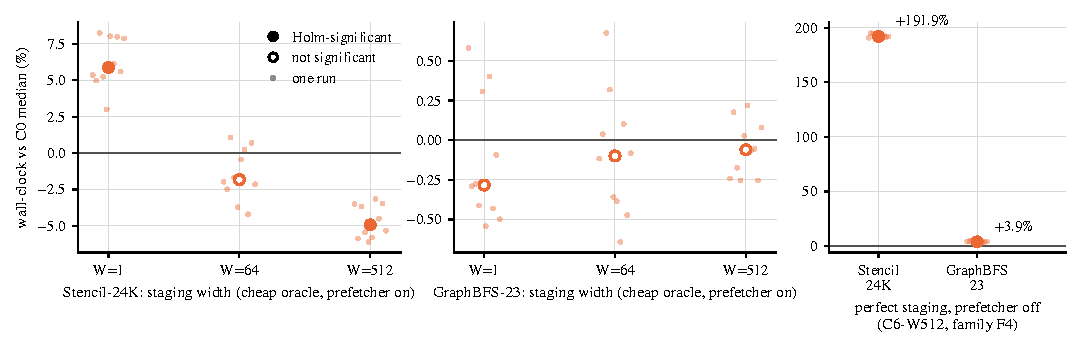
\includegraphics[width=0.95\textwidth]{figures/fig_e4_wallclock_by_arm}
\caption{RTX 5070 Ti, driver 595.91.07, stock prefetcher on: wall-clock change of the staging arms relative to the median of C0 (the shipped driver) on Stencil-24K and GraphBFS-23 (E4 family F1), and of perfect off-path staging with the in-path prefetcher off, C6-W512 (family F4, right). Each run is a point; markers are medians, filled when Holm-significant (two-sided Mann-Whitney U, n = 10 per arm). At W = 512 the Stencil-24K arm is -4.93\% against C0, while C6-W512 is +191.95\%.}
\label{fig:s-fig_e4_wallclock_by_arm}
\end{figure*}

\begin{figure*}[t]
\centering
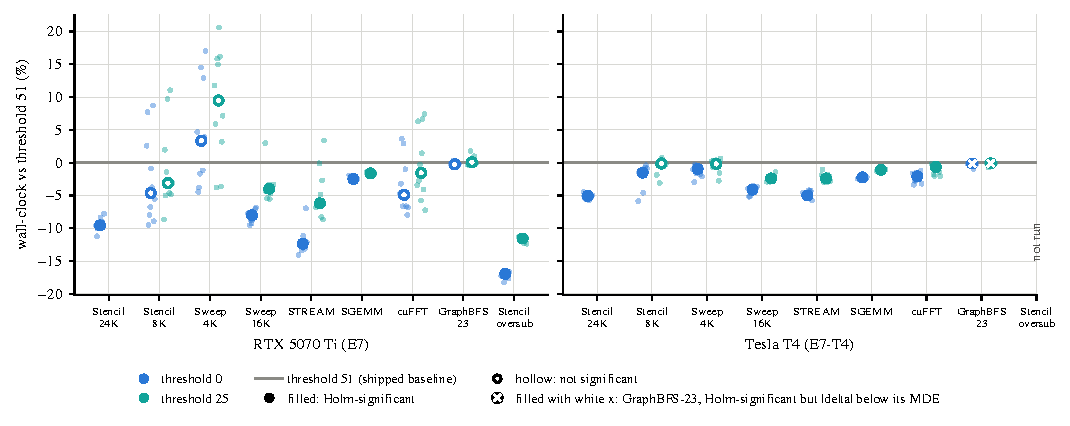
\includegraphics[width=0.95\textwidth]{figures/fig_e7_threshold_by_workload_two_platforms}
\caption{Stock driver 595.91.07, prefetcher on, no speculation: wall-clock change of threshold 0 and 25 against the shipped threshold 51 (each cell's own median), per workload, on the RTX 5070 Ti (left) and the Tesla T4 (right); the two platforms are analysed separately and not pooled. Each run is a point; markers are medians, filled when Holm-significant (two-sided Mann-Whitney U, n = 10 per cell; Stencil-24K shows threshold 0 only, from family A). The oversubscribed Stencil cell was not run on the T4. On Stencil-24K the change at threshold 0 is -9.57\% on the RTX 5070 Ti and -5.07\% on the T4, and 12 of 14 T4 family-B tests are significantly faster; GraphBFS-23's changes (0.1\% of a 54 s run) are below its minimum detectable effect (white x).}
\label{fig:s-fig_e7_threshold_by_workload_two_platforms}
\end{figure*}

\begin{figure}[t]
\centering
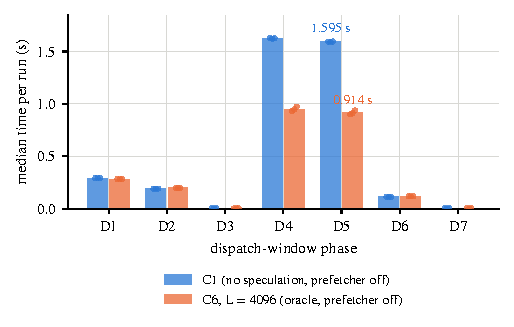
\includegraphics[width=\columnwidth]{figures/fig_ph_phase_medians}
\caption{RTX 5070 Ti, Stencil-24K, prefetcher off, E1 Part B: median time per run spent in each phase of the fault-dispatch window (D4 is the address-space lock hold and contains D5). Bars are medians, points are the runs; no statistical test is applied (n = 3 and 3). D5 is 1.595 s with C1 and 0.914 s with the oracle (C6, L = 4096).}
\label{fig:s-fig_ph_phase_medians}
\end{figure}

\begin{figure}[t]
\centering
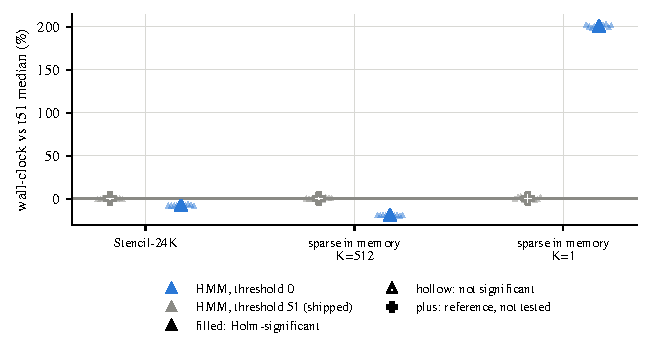
\includegraphics[width=\columnwidth]{figures/supplementary/F-H1}
\caption{RTX 5070 Ti, stock driver, system-allocated (HMM, malloc) memory, H1 Amendment 1: wall-clock of threshold 0 relative to the median at threshold 51, for Stencil-24K and the in-memory sparse benchmark at K = 512 and K = 1. Each run is a point; markers are medians, filled when Holm-significant (n = 10 per cell). At K = 1 the change is +200.52\% and on Stencil-24K -7.97\%.}
\label{fig:s-F-H1}
\end{figure}

\begin{figure}[t]
\centering
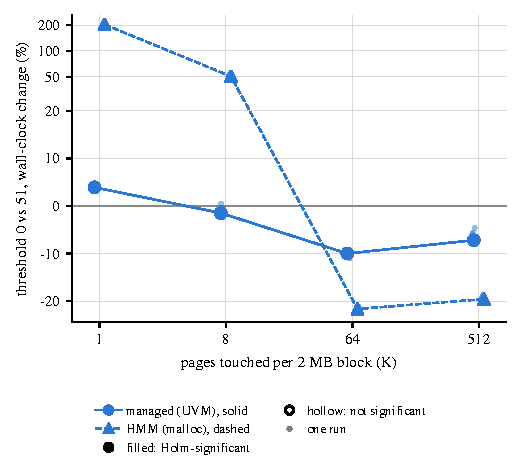
\includegraphics[width=\columnwidth]{figures/supplementary/F-H2-time}
\caption{RTX 5070 Ti, stock driver, 8 GiB array in memory: wall-clock change of threshold 0 against 51 on managed and HMM memory (panel (a) of fig\_h2\_hmm alone). Symmetric-logarithmic y axis (linear within +-20\%); each run is a point, markers are medians, filled when Holm-significant (n = 10 per cell). At K = 512 the change is -19.56\% on HMM and -7.19\% on managed memory.}
\label{fig:s-F-H2-time}
\end{figure}

\begin{figure}[t]
\centering
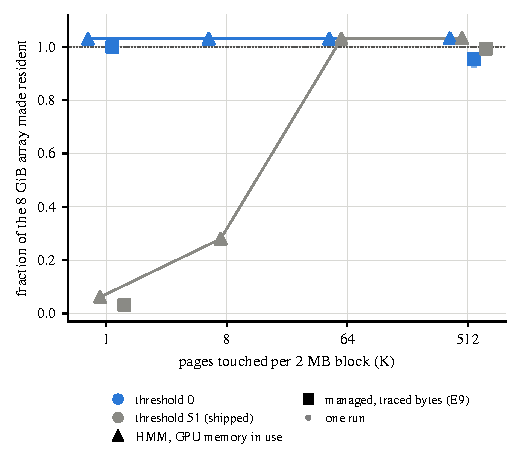
\includegraphics[width=\columnwidth]{figures/supplementary/F-H2-res}
\caption{RTX 5070 Ti, stock driver, 8 GiB array in memory: fraction of the array made resident (panel (b) of fig\_h2\_hmm alone). Two instruments from different sessions: HMM nvidia-smi memory.used (valid for 4 KB chunks) and managed nsys traced host-to-device bytes (E9, K = 1 and 512 only). Descriptive, no test; managed memory.used is not plotted because it measures allocated 2 MB chunks (catalog \#31).}
\label{fig:s-F-H2-res}
\end{figure}

\section{Artifact Catalog}
\label{sec:s3}

\subsection*{Measurement artifact catalog, v4 (updated Gate B7 correction pass)}
Eleven distinct measurement/methodology artifacts found and resolved over the course of this project (six as of the T4 GPU work block's Phase 4; five more, below, surfaced by the Gate A1/A2/B correction passes and the Gate B7 cross-platform block). Two hypotheses were investigated and explicitly \textbf{rejected} as not being real artifacts (listed at the end, for completeness -- not counted among the eleven).

\begin{table*}[t]
\centering\footnotesize
\begin{tabularx}{\textwidth}{XXXXXXXXX}
\toprule
\# & Short name & Phase found & What was mis-measured & Naive reading it would have produced & Root cause & How caught & Reached a reported result? & Evidence file \\
\midrule
1 & \textbf{Oracle cursor desync} & Phase B.1 (Gate B) & Oracle (policy=4) hit rate on every real benchmark & ``Oracle-perfect prediction gives zero benefit -- even a perfect predictor can't help, so speculation is fundamentally useless here'' & Fault trace recorded once \textbf{per demand fault}, but oracle cursor consulted once \textbf{per service batch} -- a batch coalescing \emph{k} faults consumes \emph{k} trace entries of fault stream but advances the cursor by 1, permanently desyncing after the first coalesced batch & Deliberate Gate B re-investigation with a serialized-vs-coalesced positive-control probe (\texttt{tests/\allowbreak{}hit\_\allowbreak{}probe.\allowbreak{}cu}); coalesced-probe hit rate jumped 0.0175 -> 0.4107 old-ko-vs-new-ko & \textbf{Yes} -- Phase B's original writeup (\texttt{results/\allowbreak{}phaseB/\allowbreak{}gate\_\allowbreak{}reports/\allowbreak{}gate4\_\allowbreak{}oracle.\allowbreak{}md}, \texttt{results/\allowbreak{}summary/\allowbreak{}cost\_\allowbreak{}benefit.\allowbreak{}md}) reported oracle hit\_rate=0.0000 on all 6 cells as a real finding before this was caught & \texttt{driver/\allowbreak{}PIPELINE\_\allowbreak{}FIXES.\allowbreak{}md} (FIX-1), \texttt{results/\allowbreak{}phaseB1/\allowbreak{}GATE\_\allowbreak{}B\_\allowbreak{}diagnosis.\allowbreak{}md} \\
2 & \textbf{ASLR address instability} & Phase B.1 (Gate B), found alongside \#1 & Same oracle hit-rate cells as \#1 -- an independent, compounding bug & Same naive reading as \#1 (``oracle scores zero''), reinforcing the wrong conclusion even after a cursor fix alone & \texttt{cudaMallocManaged} returns a different base VA per process; trace collection records \textbf{absolute} VAs in one process, replay happens in a \textbf{fresh} process with a different base -> zero address overlap regardless of cursor sync & Same Gate B investigation; fixed by pinning the managed-memory base with \texttt{setarch -\allowbreak{}R} across trace-collection and replay, verified stable at \texttt{0x7fffce000000} & \textbf{Yes} -- compounded with \#1 in the same originally-reported 0.0000 hit-rate cells & \texttt{driver/\allowbreak{}PIPELINE\_\allowbreak{}FIXES.\allowbreak{}md} (FIX-2), \texttt{results/\allowbreak{}phaseB1/\allowbreak{}GATE\_\allowbreak{}B\_\allowbreak{}diagnosis.\allowbreak{}md} \\
3 & \textbf{STREAM host-ordering noise} & Phase B.1 (Gate C) & STREAM wall-time delta for p1/p2/p3 vs p0 at 134M/268M element sizes & ``SpecAsync speculative prefetch gives STREAM a real -8.8\% speedup'' (a false positive \emph{in favor of} the technique) & Original runs were all-baseline-then-all-treatment (blocked ordering) on a shared EC2 instance; a slow host-noise drift or neighbor-tenant effect between the two blocks produced a spurious apparent speedup & Re-run interleaved (p0->p1->p5 alternating, 40 cycles/policy/size) plus a null-worker control (p5, enqueues but does zero lookup); the ``speedup'' flipped sign to a +1.5-2\% slowdown that p1 and p5 (null) share almost exactly, proving it is a worker-presence artifact, not prediction & \textbf{Yes} -- the -8.8\% ``speedup'' was in the original Phase B report before Gate C's interleaved re-run debunked it & \texttt{results/\allowbreak{}phaseB1/\allowbreak{}GATE\_\allowbreak{}C\_\allowbreak{}report.\allowbreak{}md} (C2) \\
4 & \textbf{T2==T3 timer collapse (``metadata \textasciitilde{}99\% of service time'')} & Phase B.1 (Gate C) & The per-batch phase breakdown (metadata vs residency) derived from T0-T4 timestamps & ``Metadata/preprocessing is the dominant cost (\textasciitilde{}99\% of service time) -- that's where async offload should target'' (wrong bottleneck attribution) & \texttt{T2} and \texttt{T3} are both set to \texttt{ktime\_\allowbreak{}get\_\allowbreak{}ns()} immediately after \texttt{service\_\allowbreak{}fault\_\allowbreak{}batch\_\allowbreak{}dispatch()} returns (same two adjacent lines), making \texttt{phase\_\allowbreak{}residency =\allowbreak{} T3-\allowbreak{}T2} identically zero; the ``metadata'' window (T1->T2) actually brackets the \emph{entire} dispatch call including residency decision and migration-push construction, not just metadata lookup & Source-level inspection of \texttt{service\_\allowbreak{}fault\_\allowbreak{}batch()}'s timer placement, cross-checked against Phase B telemetry showing \texttt{metadata\_\allowbreak{}median =\allowbreak{}=\allowbreak{} lat\_\allowbreak{}median} for every benchmark (residency always exactly 0) & \textbf{Yes} -- ``metadata ≈ 99\% of service time'' was reported as a real phase-breakdown finding before Gate C's source inspection caught the timer bug & \texttt{results/\allowbreak{}phaseB1/\allowbreak{}GATE\_\allowbreak{}C\_\allowbreak{}report.\allowbreak{}md} (C3) \\
5 & \textbf{\texttt{ring\_\allowbreak{}read\_\allowbreak{}binary} byte-offset drift} & Phase C & Decomposition-record readout past slot \textasciitilde{}1170 in any long Phase C run (\texttt{decomp\_\allowbreak{}*.\allowbreak{}bin} -> \texttt{.\allowbreak{}csv}) & Not an obviously-broken read: it would have silently produced garbled/shifted D1-D6 sub-phase values for a large fraction of batches in every workload with >1170 records (Stencil-24K, GraphBFS-23, Sweep-16K/24K all exceed this), read as noisy-but-plausible decomposition data rather than as corrupted & \texttt{ring\_\allowbreak{}read\_\allowbreak{}binary} (\texttt{specasync\_\allowbreak{}debugfs.\allowbreak{}c}) returned \texttt{to\_\allowbreak{}copy} bytes to the caller while only actually writing \texttt{floor(to\_\allowbreak{}copy/\allowbreak{}record\_\allowbreak{}size)*record\_\allowbreak{}size} bytes via \texttt{copy\_\allowbreak{}to\_\allowbreak{}user} -- the difference silently accumulated in \texttt{*ppos}, reaching exactly 32 bytes of drift by slot 1170 and misaligning every subsequent record boundary & Phase C's own \textbf{same-session} G1 accounting-closure gate (\texttt{D1+D2+svc+D6+D7 ≈ total} within ±2\%) flagged a small (<0.06\%) batch failure rate; tracing those specific failures back to the parser led to the byte-offset bug, fixed, and the run re-verified before any report was written & \textbf{No} -- caught by an automated gate check within the same Phase C session, before any garbled numbers reached \texttt{PHASEC\_\allowbreak{}REPORT.\allowbreak{}md} or any downstream figure/statistic. This is the one artifact in the catalog that was caught proactively rather than reactively (after being published), which is the point of listing it separately: the project's gate-check discipline worked as designed here & \texttt{results/\allowbreak{}phaseC/\allowbreak{}PHASEC\_\allowbreak{}REPORT.\allowbreak{}md} (``Root-Cause Note: ring\_read\_binary Fix'', ``G1 — Accounting Closure'') \\
6 & \textbf{cuFFT hit-rate blocked-protocol outlier (25.47\%)} & Phase B (pre-fix sweep), caught at Task T2 (T4 GPU work block) & cuFFT hit rate at policy=2 (stride), depth=0, prefetch ON, size=67,108,864 (\texttt{phaseB\_\allowbreak{}telemetry.\allowbreak{}csv}) & ``SpecAsync's stride predictor gets real traction on cuFFT's large-stride access pattern -- the one real workload where the hit-table mechanism demonstrably works, distinct from the near-zero rates on Stencil/GraphBFS/SGEMM/STREAM'' (a false positive suggesting cuFFT was a favorable case for the mechanism) & The 25.47\% figure was measured in a \textbf{single, non-interleaved, uncontrolled run} during Phase B's pre-fix sweep (\texttt{CUFFT\_\allowbreak{}PROVENANCE.\allowbreak{}md}: ``cuFFT ran on the T4 only during the pre-fix Phase B sweep'') -- structurally the same failure mode as artifact \#3 (STREAM host-ordering noise): a blocked/single-shot measurement with no interleaving to control for host noise, drift, or a favorable transient & Task T2's interleaved rerun (15 clean reps at the exact matching policy/depth/prefetch/size configuration) measured 4.07\% aggregate hit rate -- a sixth of the legacy figure -- with no accompanying wall-clock benefit at any of the three tested sizes & \textbf{Yes} -- the 25.47\% figure was already in circulation in \texttt{phaseB\_\allowbreak{}telemetry.\allowbreak{}csv} and cited in \texttt{CUFFT\_\allowbreak{}PROVENANCE.\allowbreak{}md}'s own provenance audit (correctly, as a real T4/595.71.05 measurement) before Task T2's controlled rerun showed it does not reproduce. Unlike artifact \#5, this was not caught by an automated gate -- it required a dedicated interleaved rerun task to surface, which is exactly why \texttt{CUFFT\_\allowbreak{}PROVENANCE.\allowbreak{}md} flagged the cell as needing revisiting rather than treating the number as settled & \texttt{results/\allowbreak{}analysis/\allowbreak{}GATE\_\allowbreak{}T2\_\allowbreak{}REPORT.\allowbreak{}md}, \texttt{results/\allowbreak{}figures/\allowbreak{}CUFFT\_\allowbreak{}PROVENANCE.\allowbreak{}md}, \texttt{results/\allowbreak{}figures/\allowbreak{}exclusion\_\allowbreak{}manifest.\allowbreak{}csv} (cuFFT/67108864/p2/hit\_rate row) \\
7 & \textbf{Ring saturation without wraparound} & T4 GPU work block, Task T4 (\texttt{t4\_\allowbreak{}prefetch\_\allowbreak{}off\_\allowbreak{}telemetry.\allowbreak{}sh}'s pre-fix \texttt{run\_\allowbreak{}c1/\allowbreak{}c2/\allowbreak{}c3\_\allowbreak{}block}) & Absolute demand-fault/enqueue/drop/hit counts read from \texttt{specasync\_\allowbreak{}log} across 15 reps per config & ``Real workloads sustain 70.6M (Stencil-24K) / 24.9M (GraphBFS-23) demand faults across 15 independent repetitions'' -- treating 15 separately-dumped \texttt{.\allowbreak{}bin} files as 15 independent per-rep totals & \texttt{specasync\_\allowbreak{}log} is a fixed 131,071-record ring that was never cleared between reps (bug in the per-rep loop, since fixed). Once full, it \textbf{stops recording new activity rather than wrapping}, so every dump taken after saturation is a byte-for-byte-identical copy of the same frozen snapshot, not that rep's own data. Stencil-24K saturates during rep 2 of 15 (14 of 15 kept-rep dump files identical; only 2 distinct observations exist); GraphBFS-23 saturates during rep 5 of 15 (11 of 15 identical; 5 distinct observations exist) & First flagged as an ``open item'' in \texttt{GATE\_\allowbreak{}A1\_\allowbreak{}REPORT.\allowbreak{}md} (its own properly-cleared-per-rep counters showed roughly an order-of-magnitude discrepancy against \texttt{GATE\_\allowbreak{}T4\_\allowbreak{}REPORT.\allowbreak{}md}'s totals); confirmed and precisely quantified by direct \texttt{.\allowbreak{}bin} inspection in \texttt{GATE\_\allowbreak{}T4\_\allowbreak{}REPORT.\allowbreak{}md}'s 2026-08-12 correction note; a later correction pass (2026-08-13) parsed the surviving pre-saturation \texttt{.\allowbreak{}bin} files directly to derive a genuinely clean per-rep fault rate & \textbf{Yes} -- the inflated absolute counts, and a derived rate built from them (see artifact \#8), were both published as findings in \texttt{GATE\_\allowbreak{}T4\_\allowbreak{}REPORT.\allowbreak{}md} before being caught & Left the ratio-based \texttt{hit\_\allowbreak{}rate} conclusion valid (numerator and denominator over-count together, so the ratio is unaffected) but corrupted every absolute-count-derived figure, most importantly the fault-rate calculation feeding artifact \#8 & \texttt{GATE\_\allowbreak{}T4\_\allowbreak{}REPORT.\allowbreak{}md} (correction note + updated Section 2), \texttt{GATE\_\allowbreak{}A1\_\allowbreak{}REPORT.\allowbreak{}md} (open item + Result 2) \\
8 & \textbf{Rate-arithmetic 15x aggregation error} & T4 GPU work block, Part 2 verification (\texttt{RATE\_\allowbreak{}MISMATCH\_\allowbreak{}VERIFICATION.\allowbreak{}md}) & The ``faults/second'' rate derived from \texttt{GATE\_\allowbreak{}T4\_\allowbreak{}REPORT.\allowbreak{}md} Section 1's totals & ``Real workloads sustain 0.4-4.7 million demand faults/second, so the speculative worker essentially never wins the race'' -- an overstated mismatch (the qualitative direction happened to still be correct, by luck, not by a sound calculation) & Divided the fault total \textbf{summed across all 15 repetitions} by \textbf{one repetition's} wall-clock duration (the same 15s/58s figures the surrounding sentence itself cited as the ``15-58 seconds of wall-clock time'' range) instead of the cumulative 15-rep wall-clock time -- inflated the rate by very close to 15x, the repetition count & A dedicated Part 2 verification pass (\texttt{RATE\_\allowbreak{}MISMATCH\_\allowbreak{}VERIFICATION.\allowbreak{}md}) reconstructed the dispatch-granularity argument from source and cross-checked totals against \texttt{GATE\_\allowbreak{}T4\_\allowbreak{}REPORT.\allowbreak{}md} before recomputing the rate independently & \textbf{Yes} -- published in \texttt{GATE\_\allowbreak{}T4\_\allowbreak{}REPORT.\allowbreak{}md} Section 2 as a quantified mechanism finding (``essentially never wins the race'') before being caught. This entry resolves the ``decision point'' a prior version of this catalog left open (whether an arithmetic error, as opposed to a measurement/protocol confound, belongs here) -- given it reached a published result and compounds with artifact \#7 on the exact same figure, it is catalogued rather than left as a methodology-section footnote & This ``corrected'' rate was \textbf{itself still \textasciitilde{}15x too high}, since its numerator inherited artifact \#7's ring-duplication problem, not yet known when this correction was written -- doubly corrected in a later pass (2026-08-13, see \texttt{GATE\_\allowbreak{}T4\_\allowbreak{}REPORT.\allowbreak{}md}/\texttt{GATE\_\allowbreak{}A1\_\allowbreak{}REPORT.\allowbreak{}md}'s current sections) & \texttt{RATE\_\allowbreak{}MISMATCH\_\allowbreak{}VERIFICATION.\allowbreak{}md} (intermediate correction, now itself superseded), \texttt{GATE\_\allowbreak{}T4\_\allowbreak{}REPORT.\allowbreak{}md}/\texttt{GATE\_\allowbreak{}A1\_\allowbreak{}REPORT.\allowbreak{}md} (current, doubly-corrected figures) \\
9 & \textbf{Ceiling units mismatch} & This session, Gate B7 cross-platform block (\texttt{CEILING\_\allowbreak{}BASIS\_\allowbreak{}VERIFICATION.\allowbreak{}md}) & End-to-end pipelining ceiling (\texttt{GATE\_\allowbreak{}T3\_\allowbreak{}REPORT.\allowbreak{}md}'s 6-workload extension, and Gate B7's 5070 Ti rerun, which deliberately copied the same formula) & ``Up to 19\% (T4) / 29\% (RTX 5070 Ti) of wall-clock time could be recovered by hiding D1+D2'' -- and, downstream, a false cross-platform divergence (``this platform's ceiling runs notably higher than the T4's at large sizes'') & Summed the dispatch-window numerator across all 5 trials while dividing by only \textbf{one} trial's median wall-clock -- a units mismatch that inflates the ratio by a factor mechanically close to the trial count (\textasciitilde{}5x) & A verification pass requested to test a \emph{different} hypothesis (batch overlap inflating the numerator -- refuted directly, 0/N adjacent batches overlap on either platform) instead found the formula produces \textbf{mathematically impossible >100\% window/wall-clock fractions} on 4 of 6 T4 workloads under a span-based numerator -- proof the formula was wrong, not merely suspiciously large & \textbf{Yes} -- published in \texttt{GATE\_\allowbreak{}T3\_\allowbreak{}REPORT.\allowbreak{}md} and this session's \texttt{GATE\_\allowbreak{}B7\_\allowbreak{}5070TI\_\allowbreak{}PHASEC.\allowbreak{}md}, including a specific cross-platform ``diverges at the high end'' finding that did not survive the correction (the corrected convention \textbf{reverses} it: the T4 runs higher than the 5070 Ti at 5 of 6 workloads) & Inflated every published ceiling \textasciitilde{}5x on both platforms; the cross-platform divergence finding was entirely an artifact of this bug, not a real platform difference & \texttt{CEILING\_\allowbreak{}BASIS\_\allowbreak{}VERIFICATION.\allowbreak{}md}, \texttt{GATE\_\allowbreak{}T3\_\allowbreak{}REPORT.\allowbreak{}md}/\texttt{GATE\_\allowbreak{}B7\_\allowbreak{}5070TI\_\allowbreak{}PHASEC.\allowbreak{}md}/\texttt{PIPELINING\_\allowbreak{}CEILING.\allowbreak{}md}/\texttt{CLAIM\_\allowbreak{}SCOPE.\allowbreak{}md} correction notes \\
10 & \textbf{\texttt{setarch -\allowbreak{}R} regime effect} & This session, Gate A2/A2b & \texttt{ASLR\_\allowbreak{}OFF} wall-clock variance and speculative-volume variance, Stencil-24K, oracle policy (C3) & Not a false conclusion in the usual sense -- a \textbf{methodological property of oracle-based evaluation} that, if unstated, would let a reader assume T1's \texttt{setarch -\allowbreak{}R}-pinned results reflect general platform noise rather than a regime specifically tied to running the speculative pipeline with a fixed allocation address & Oracle replay (policy=4) requires a fixed \texttt{cudaMallocManaged} base address for trace-address alignment across collect/replay sessions, so every oracle-based run in this project necessarily uses \texttt{setarch -\allowbreak{}R}. \texttt{GATE\_\allowbreak{}A2B\_\allowbreak{}SETARCH\_\allowbreak{}REGIME.\allowbreak{}md} (pre-registered, C1-vs-C3 split test) found the \texttt{ASLR\_\allowbreak{}ON}/\texttt{ASLR\_\allowbreak{}OFF} wall-clock and speculative-volume variance difference is \textbf{absent in C1} (no speculation, p=0.970 location, p=0.179 spread) but \textbf{present and large in C3} (oracle): Levene's test stat=10.659, p=0.0043, variance ratio (OFF/ON) = \textbf{522.7x}, reproducing \texttt{GATE\_\allowbreak{}A2\_\allowbreak{}REPORT.\allowbreak{}md}'s original finding closely on an independent n=10/arm sample two days later & Deliberately investigated, not stumbled into -- \texttt{GATE\_\allowbreak{}A2\_\allowbreak{}REPORT.\allowbreak{}md} first flagged the ASLR-correlated volume difference as ``a secondary, unplanned observation... outside this task's scope to chase further''; \texttt{GATE\_\allowbreak{}A2B\_\allowbreak{}SETARCH\_\allowbreak{}REGIME.\allowbreak{}md} was pre-registered specifically to test whether it was general (would implicate T1) or speculation-specific (would not) & \textbf{No} -- caught by design, before any claim depending on the distinction was published. Listed here as a methodological property to disclose, not a bug that produced a wrong number & T1 (platform-of-record) is not contaminated by a general paging artifact (C1's null result rules that out), but its reported run-to-run variance should be read as characteristic of the \texttt{ASLR\_\allowbreak{}OFF} speculative regime specifically, not general instance noise -- a manuscript methods/limitations sentence, not a retraction & \texttt{GATE\_\allowbreak{}A2\_\allowbreak{}REPORT.\allowbreak{}md}, \texttt{GATE\_\allowbreak{}A2B\_\allowbreak{}SETARCH\_\allowbreak{}REGIME.\allowbreak{}md} \\
11 & \textbf{Host memory leak as a run-order confound} & This session, Gate B6 (\texttt{HOST\_\allowbreak{}MEMORY\_\allowbreak{}LEAK\_\allowbreak{}5070TI.\allowbreak{}md}) & \texttt{MemAvailable} across any session of repeated (module reload + CUDA run) cycles on the RTX 5070 Ti / driver 595.84 host & Not a false conclusion produced yet -- a \textbf{candidate, unconfirmed contributor} to an already-published finding (B5's run-order wall-clock drift, rho=0.548, p=0.0123) that, if not flagged, could be mistaken for a settled platform property rather than a live open question & Reproducible \textasciitilde{}244MB leaked per (module-reload + CUDA-run) cycle, confirmed to reproduce at the same rate on the \textbf{stock, unpatched} NVIDIA 595.84 driver (not a SpecAsync defect -- an upstream driver issue), monotonic across a session (not per-run noise), lands in \texttt{/\allowbreak{}proc/\allowbreak{}meminfo}'s unaccounted pool (not reclaimable via \texttt{drop\_\allowbreak{}caches}) & A dedicated characterization pass (4 conditions x n≥5 cycles, batch-overlap-style controlled comparison against the stock driver) run specifically because Task 4's cuFFT rerun hit a near-OOM condition mid-session -- the leak was severe enough to force a stop-and-characterize before continuing, not found by a passive audit & \textbf{Partially} -- the leak itself was not previously reported as a finding (it caused an operational stop, not a wrong number in a report), but B5's drift finding it may help explain was already published without this candidate mechanism attached & Flagged explicitly as \textbf{candidate, not proven} -- Task 3 (this platform's non-reproduction of B5's drift) is equally consistent with plain session-to-session noise; the leak explanation is offered alongside, not in place of, that simpler account & \texttt{HOST\_\allowbreak{}MEMORY\_\allowbreak{}LEAK\_\allowbreak{}5070TI.\allowbreak{}md}, \texttt{GATE\_\allowbreak{}B6\_\allowbreak{}TASK3\_\allowbreak{}A2\_\allowbreak{}REPLICATION.\allowbreak{}md} (addendum) \\
\bottomrule
\end{tabularx}
\end{table*}

\subsection*{Second occurrence of artifact \#7 (Gate B9, 2026-08-15)}
\textbf{The fix applied to \texttt{t4\_\allowbreak{}prefetch\_\allowbreak{}off\_\allowbreak{}telemetry.\allowbreak{}sh} addressed one script; the exposure is architectural.} Any script that reads \texttt{specasync\_\allowbreak{}log} (or \texttt{specasync\_\allowbreak{}decomp\_\allowbreak{}log}, or \texttt{specasync\_\allowbreak{}worker\_\allowbreak{}log} -- all three are the same 131,072-slot, drop-on-full ring design) a single time at the end of a run, rather than clearing and re-reading periodically, inherits this artifact regardless of whether the per-rep-clear bug that caused the \emph{first} occurrence is present or not. \texttt{tests/\allowbreak{}t\_\allowbreak{}b9\_\allowbreak{}task2\_\allowbreak{}mechanism.\allowbreak{}sh} (Gate B9 Task 2, C1-vs-C3 mechanism instrumentation at \textasciitilde{}1.08x oversubscription, N=48000/iters=20) did clear the ring correctly between every rep -- and still saturated \textbf{within every single one of its 20 kept runs}, because a single rep's fault volume at this oversubscription level vastly exceeds ring capacity on its own; no cross-rep contamination was needed to trigger it this time.

Two new details this occurrence adds, not present in the original:

\begin{enumerate}
\item \textbf{Different arms saturating at the same record count is not evidence of equal coverage.} C1 and C3 both hit exactly 131,071 records in all 20/20 runs -- but C1's run took \textasciitilde{}161s and C3's took \textasciitilde{}69s, so the captured window covers \textbf{2.8\% of C1's run} versus \textbf{7.9\% of C3's run} (measured directly from each snapshot's \texttt{t0\_\allowbreak{}ns}/\texttt{t4\_\allowbreak{}ns} span against the run's wall-clock). A naive between-arm comparison of ring-derived totals (here, \texttt{total\_\allowbreak{}demand\_\allowbreak{}faults}: C3 appeared to have +11.5\% more than C1) silently compares different \emph{fractions} of two runs of very different length, not the same slice of comparable work. The direction of the apparent difference cannot be trusted without first establishing the arms are looking at the same relative window, which in general they are not once either ring saturates.
\item \textbf{Not all rings saturate the same way, and the ones that don't can point the opposite direction.} \texttt{specasync\_\allowbreak{}fault\_\allowbreak{}trace} (the demand-fault address ring used for the thrash/re-migration proxy) is a genuine circular \emph{overwrite} buffer with no drop-on-full behavior -- it holds the \textbf{trailing} window of a run once its 1,048,576-slot capacity is exceeded, which it was in all 20/20 runs here too. So in the same Gate B9 Task 2 run, the batch/decomp/work-ring metrics reflected the first \textasciitilde{}3-8\% of each run and the trace-ring metric reflected the last portion -- two telemetry sources from the \emph{same} run, covering \emph{disjoint} and \emph{non-overlapping} time windows, neither comparable to the other nor to the run as a whole.
\end{enumerate}
Caught before any figure was published (Task 2's demand-fault comparison was flagged and withheld pending a redesigned periodic-drain harness rather than reported), but it is the second time this exact architectural gap has produced a plausible-looking, wrong headline number from otherwise-correct per-rep instrumentation. See \texttt{GATE\_\allowbreak{}B9\_\allowbreak{}OVERSUB\_\allowbreak{}MECHANISM.\allowbreak{}md} (once written) for the drain-harness redesign and its validation.

\subsection*{Decision point (RESOLVED 2026-08-13): does the rate-arithmetic error belong in this catalog?}
\textbf{Resolved: yes, as artifact \#8.} This entry originally deferred the choice between adding the \texttt{GATE\_\allowbreak{}T4\_\allowbreak{}REPORT.\allowbreak{}md} rate-arithmetic error as a new ``analysis arithmetic error'' category (Option A) or leaving it as a methodology-section footnote only (Option B), on the grounds that it was ``different in kind'' from artifacts \#1-6 -- a bookkeeping error downstream of correct measurements, not a wrong measurement itself. Two things changed the calculus: first, that same figure turned out to be wrong \textbf{twice}, compounding with the independently-discovered artifact \#7 (ring saturation) on the exact same headline number -- a single footnote could not represent that compounding relationship as clearly as two linked catalog entries can. Second, this pass added three more entries (9, 10, 11) that also don't fit the original ``wrong measurement, correctly recorded but misinterpreted'' mold cleanly (\#9 is also a pure downstream arithmetic error; \#10 is not an error at all, just a methodological property worth disclosing) -- the catalog's working definition has already broadened past the original six's shape. Kept in, not deferred further.

\subsection*{Synthesis: what artifacts \#7-9 have in common}
\textbf{Artifacts \#7, \#8, and \#9 share a pattern worth stating explicitly: each was caught by an independent verification pass, not by the original analysis that produced the number, and each inflated an absolute or derived headline figure while leaving a \emph{ratio} computed from the same underlying data intact.} \#7's ring duplication left \texttt{hit\_\allowbreak{}rate} (hits/enqueued) valid while corrupting absolute fault/enqueue counts. \#8's denominator error left the underlying fault and wall-clock totals individually correct while corrupting the rate computed from them. \#9's trial-aggregation error left D1+D2 \emph{share} (which uses the same aggregation on both its own numerator and denominator, so the units-mismatch factor cancels) valid while corrupting the window/wall-clock ratio and everything downstream of it. In every case, none of these were caught by the original analysis, or by peer review of the resulting report -- each required someone to come back with a specific, adversarial question (``does this number survive a sanity bound?'', ``what happens if I recompute this from a different angle?'') rather than trusting a plausible-looking result.

\textbf{A sharper lesson sits inside artifact \#8 specifically, worth stating on its own: a verification pass that reuses an upstream aggregation inherits that aggregation's defects.} \texttt{RATE\_\allowbreak{}MISMATCH\_\allowbreak{}VERIFICATION.\allowbreak{}md} was itself a dedicated verification pass -- it caught and fixed the 15x denominator error carefully, cross-checking its inputs against \texttt{GATE\_\allowbreak{}T4\_\allowbreak{}REPORT.\allowbreak{}md}'s published totals before recomputing. But ``cross-checking against the published totals'' was exactly the mistake: those totals were themselves artifact \#7's ring-duplicated sum, and a match against a wrong number is not validation. The verification pass corrected the arithmetic it was looking for (the division) while silently carrying forward the one input it never re-derived from source (the numerator) -- so its own ``corrected'' rate was still wrong, by nearly the same order of magnitude the first error was, and stayed that way until a second pass parsed the raw \texttt{.\allowbreak{}bin} ring dumps directly instead of trusting any prior report's aggregate figure, including the verification pass's own. \textbf{The lesson is not ``verify twice'' -- two independent passes both reused the same corrupted upstream number and both produced a plausible-looking result.} It is that a verification pass only protects against the specific failure mode it was designed to catch; any input it takes as given, rather than re-deriving from the rawest available source, can carry a different, unrelated defect straight through the correction. This is the concrete argument for verification passes as methodology, not just as cleanup: three of this project's headline quantitative claims (a real-workload fault rate, an end-to-end pipelining ceiling, and -- earlier in the project's history -- the STREAM speedup and metadata-dominance findings, artifacts \#3-4) were wrong in ways that looked entirely plausible until specifically checked, and stayed in circulation, cited by other reports, until a dedicated pass went looking.

\subsection*{Hypotheses investigated and rejected (not counted among the six)}
These were suspected artifacts that, on investigation, turned out \textbf{not} to be real — included here so the catalog documents the negative results too, not just the confirmed bugs.

\begin{table*}[t]
\centering\footnotesize
\begin{tabularx}{\textwidth}{XXXX}
\toprule
Hypothesis & Why suspected & Verdict & Evidence \\
\midrule
Hit-accounting counter is broken (\texttt{spec\_\allowbreak{}hits} never fires) & Near-zero hit rates on every real benchmark looked like a broken counter & \textbf{REJECTED} -- a deterministic positive control (\texttt{tests/\allowbreak{}hit\_\allowbreak{}probe.\allowbreak{}cu}, serialized, prefetch off) scored 254/256 = 99.2\%; the counter is sound. Near-zero hit rates on real benchmarks are a real interaction with the UVM prefetcher + per-batch (not per-fault) prediction, not instrumentation failure & \texttt{driver/\allowbreak{}PIPELINE\_\allowbreak{}FIXES.\allowbreak{}md} (FIX-0), \texttt{results/\allowbreak{}phaseB1/\allowbreak{}GATE\_\allowbreak{}A\_\allowbreak{}report.\allowbreak{}md} \\
Oracle replay is O(n²) in trace length & Phase B's original sweep reported the oracle ``up to 100x slower''; a quadratic scan was the leading hypothesis & \textbf{REJECTED} -- \texttt{specasync\_\allowbreak{}oracle\_\allowbreak{}next\_\allowbreak{}addr()} is an O(1) atomic post-increment cursor with modulo wraparound; no per-fault linear scan exists anywhere in the replay path. If a real slowdown exists, it is not this & \texttt{results/\allowbreak{}phaseB1/\allowbreak{}GATE\_\allowbreak{}B\_\allowbreak{}diagnosis.\allowbreak{}md} (H1) \\
\bottomrule
\end{tabularx}
\end{table*}

\medskip\hrule\medskip
\subsection*{Entries \#12–\#25 (applied 2026-10-05, Gate C1-APPLY)}
Appended from \texttt{results/\allowbreak{}analysis/\allowbreak{}consolidation/\allowbreak{}ARTIFACT\_\allowbreak{}CATALOG\_\allowbreak{}ADDITIONS\_\allowbreak{}PROPOSED.\allowbreak{}md}. The original table above is unchanged; the two amendments below amend its rows.

\subsection*{Entries}
\subsubsection*{\#12 · Comparison against a crippled baseline \emph{(promoted; long-standing candidate)}}
\begin{itemize}
\item \textbf{What happened (Gate B9):} Task 2b compared the oversubscription oracle arm (C3) only against C1, which has speculation off \textbf{and} the prefetcher off. C3 was 54.00\% faster at iters = 20, Holm-significant across all five iteration values, which fired the project's primary falsification trigger. The verification pass added C0, the system as shipped, and C3 was \textbf{1.76–4.47× slower than C0} at every iteration value.
\item \textbf{False conclusion it would have produced:} ``Speculation delivers a large, decisive oversubscription speedup'', reversing the paper's central negative claim on the strength of a comparison against a configuration nobody runs.
\item \textbf{How caught:} an \textbf{independent verification pass}, required by standing policy whenever a falsification trigger fires (\texttt{OVERSUB\_\allowbreak{}C3\_\allowbreak{}VERIFICATION.\allowbreak{}md}). The pass explicitly flagged this as ``a different failure mode … a correct measurement answering the wrong question''.
\item \textbf{Evidence:} \texttt{B9.\allowbreak{}2c.\allowbreak{}iters1} … \texttt{B9.\allowbreak{}2c.\allowbreak{}iters20}: C3 vs C0 +447.43\% to +176.45\%, all Holm-significant; C1 = 159.67 s vs C0 = 27.18 s at iters 20.
\item \textbf{Family:} Validation that could not fail. Beating a baseline built to be beaten is a test with almost no power to disappoint.
\item \textbf{Standing consequence:} ``baselines named explicitly'' became a standing rule, and every Gate E pre-registration names C0 and C1 separately.
\end{itemize}
\subsubsection*{\#13 · Oracle recording/consumption granularity mismatch, with a diagnosis that mislabelled the recording side}
\begin{itemize}
\item \textbf{What happened (Gate E0 §1, §7; E0.5 Addition 1):}
\begin{itemize}
\item The oracle trace is \textbf{recorded once per va-block dispatch group} (the first coalesced fault of each group), but \textbf{consumed once per coalesced fault}.
\item The replay cursor therefore runs \textasciitilde{}11.7× (Stencil-24K) / \textasciitilde{}2.1× (GraphBFS-23) faster than the trace was recorded, and it wraps several times during a single replay.
\item FIX-1 (\texttt{cc90fc1}) introduced the full magnitude; \texttt{fc384fb} only redistributed it (E0.5 Addition 1 corrected the prior attribution).
\end{itemize}
\item \textbf{False conclusion it would have produced (and did):} every C3 result was read as ``against a maximally favorable, oracle-perfect predictor'' (T1, T4/A1, B5–B7, B9, B10; CS 6/7/8/10). \textbf{No oracle measurement before E0.5 used aligned recording and consumption.}
\item \textbf{Amendment to existing \#1:} \#1's root-cause text says the trace was "recorded once \textbf{per demand fault}". E0 §1 shows it was recorded once per \textbf{dispatch group}. \#1's fix therefore addressed the wrong granularity and left this mismatch in place. Propose amending \#1's root-cause cell to point to \#13.
\item \textbf{How caught:} an \textbf{independent source audit} (Gate E0), 103 days after FIX-1 (\texttt{cc90fc1}, 2026-06-13; the audit commit \texttt{e7de063}, 2026-09-24), by tracing the consumption loop rather than trusting the recording side's description.
\item \textbf{Evidence:} 11.7× / 2.1× and the wrap counts are \textbf{PROSE-ONLY} (E0 §7; E0.5). The post-fix 1:1 alignment (2,953,867 = 2,953,867 and 483,896 = 483,896) is also \textbf{PROSE-ONLY} (E0.5 Step 5; raw traces gitignored).
\item \textbf{Family:} Aggregation-level mismatch. This is the most consequential instance: one quantity recorded at one level and consumed at another.
\end{itemize}
\subsubsection*{\#14 · A positive control that could not fail}
\begin{itemize}
\item \textbf{What happened:} three instances.
\begin{enumerate}
\item The \textbf{serialized} hit probe (\texttt{tests/\allowbreak{}hit\_\allowbreak{}probe.\allowbreak{}cu}: one fault per service batch, by construction, with a full \texttt{cudaDeviceSynchronize()} between touches) scored 0.99 on \textbf{both} the buggy and the fixed module. \texttt{PIPELINE\_\allowbreak{}FIXES.\allowbreak{}md:57-\allowbreak{}63}: "The old code scores high on the \emph{serialized} probe only by a degenerate 'self-hit': it tags the page that is \emph{currently} faulting (zero lead time)." With one fault per batch, recording and consumption granularity coincide, so the probe structurally cannot see \#13.
\item The \textbf{coalesce} probe used to validate FIX-1 had k ≈ 1 dispatch groups per coalesced fault (442 faults / 450 trace entries). So it did not exercise dispatch-group collapsing either (E0.5 Addition 2: ``cannot distinguish 'cursor desync fixed' from 'still broken for an unrelated reason''').
\item \textbf{Recurrence, caught in time:} in E3b Step 2, \texttt{group\_\allowbreak{}probe}'s width checks ("\texttt{spec\_\allowbreak{}pages\_\allowbreak{}requested} ≈ W × calls") held \textbf{trivially}, as 0 = W × 0, because the worker never reached \texttt{make\_\allowbreak{}resident} in that probe.
\end{enumerate}
\item \textbf{False conclusion it would have produced:}
\begin{itemize}
\item Instances 1–2: ``FIX-1 fixed the oracle; the hit-accounting path is sound'' (the catalog's own rejected-hypothesis row relies on instance 1).
\item Instance 3: ``the width path is regression-tested''.
\end{itemize}
\item \textbf{How caught:}
\begin{itemize}
\item Instances 1–2 were caught by an \textbf{independent later pass} (E0.5), although instance 1's degeneracy was already written in the original fix note's own footnote and not acted on.
\item Instance 3 was caught by \textbf{the original analysis}, in the same step, because the counters were read with the question ``was the path exercised at all?''. It was recorded before Step 3 relied on it.
\end{itemize}
\item \textbf{Amendment to the rejected-hypothesis row} ("\texttt{spec\_\allowbreak{}hits} never fires" → REJECTED): the probe proves the counter \emph{fires}. Its 254/256 = 99.2\% includes zero-lead self-hits on old code, and what the counter measures is a 10 ms window (\#20). Propose narrowing the verdict to ``fires as coded; see \#14 and \#20''.
\item \textbf{Evidence:}
\begin{itemize}
\item 254/256, 0.99/0.99, 442/450 and 56 enqueued are \textbf{PROSE-ONLY} (\texttt{GATE\_\allowbreak{}A\_\allowbreak{}report.\allowbreak{}md}, \texttt{PIPELINE\_\allowbreak{}FIXES.\allowbreak{}md}, E0.5).
\item Instance 3: \texttt{results/\allowbreak{}analysis/\allowbreak{}gate\_\allowbreak{}e/\allowbreak{}e3b/\allowbreak{}step2\_\allowbreak{}runs.\allowbreak{}csv} (\texttt{spec\_\allowbreak{}migrations =\allowbreak{} 0}, \texttt{spec\_\allowbreak{}pages\_\allowbreak{}requested =\allowbreak{} 0} in all six rows). That is a committed derived file, not in the extract because it was read directly.
\end{itemize}
\item \textbf{Family:} Validation that could not fail.
\end{itemize}
\subsubsection*{\#15 · A relative improvement accepted without an absolute ceiling}
\begin{itemize}
\item \textbf{What happened (E0.5):} FIX-1 was validated as ``23× more hits'' on the coalesce probe: \textbf{1 → 23} hits, out of 57 and 56 enqueued. That is an absolute difference of 22 events. The expected ceiling for that probe was never computed.
\item \textbf{False conclusion it would have produced (and did):} ``FIXED and verified'' (\texttt{PIPELINE\_\allowbreak{}FIXES.\allowbreak{}md}), which licensed every later oracle result.
\item \textbf{How caught:} an \textbf{independent pass} (E0.5, ``FIX-1's validation rested on single-digit counts'').
\item \textbf{Evidence:} 1/57, 23/56 and 22 events are \textbf{PROSE-ONLY} (E0.5; raw \texttt{oracle\_\allowbreak{}coalesce/\allowbreak{}*.\allowbreak{}bin} gitignored).
\item \textbf{Family:} Validation that could not fail (a ratio of small counts has no power).
\end{itemize}
\subsubsection*{\#16 · Denominator mismatch: per-enqueued hit rate against a per-fault ceiling}
\begin{itemize}
\item \textbf{What happened (E0.5 Addendum §3; CS row 6):}
\begin{itemize}
\item CS 6's ``\textasciitilde{}1/coalesce\_factor'' ceiling (≈12.7\% for 7.9 faults per batch) bounds \textbf{how many faults receive a prediction}.
\item The reported 41.07\% measures \textbf{success among the 56 predictions made} (hits ÷ enqueued).
\item The claim's own evidence ``exceeds [the] ceiling by more than 3x'' only because the two use different denominators.
\end{itemize}
\item \textbf{False conclusion it would have produced:} ``the one-prediction-per-batch design caps the hit rate at \textasciitilde{}1/coalesce\_factor'', a mechanistic claim stated as following ``directly'' from the fix.
\item \textbf{How caught:} an \textbf{independent pass} (E0.5), by recomputing both quantities from the raw ring.
\item \textbf{Evidence:} 12.7\%, 41.07\%, 56 and 442 are \textbf{PROSE-ONLY}. The project-wide convention (hits ÷ enqueued) is confirmed against \texttt{T4hit.\allowbreak{}*}: for example GraphBFS 51,569 / 20,505,109 = 0.2515\% (\texttt{T4hit.\allowbreak{}bench\_\allowbreak{}graph\_\allowbreak{}bfs.\allowbreak{}repALL\_\allowbreak{}15\_\allowbreak{}SUMMED.\allowbreak{}superseded\_\allowbreak{}multicounted}).
\item \textbf{Family:} Aggregation-level mismatch (E0.5 calls it ``a fourth instance … alongside artifacts \#7, \#8, \#9'').
\end{itemize}
\subsubsection*{\#17 · Index drift: duplicate-fault counts vary run to run and silently break index-based replay}
\begin{itemize}
\item \textbf{What happened (E0.8; corrected in E0.9 §1):} the first-touch order of pages is nearly identical across runs (Stencil-24K: at most 107 ranks of 1,125,000). The \textbf{number of duplicate faults per page} differs by 1,247–4,418 between plain C1 runs. Any position-anchored comparison therefore drifts, and positional accuracy swings between \textasciitilde{}0\% and \textasciitilde{}100\% with the sign of the drift.
\item \textbf{False conclusion it would have produced (and did, for one gate):} E0.7's ``Stencil-24K is closer to genuine divergence'', which would have abandoned trace replay for the wrong reason.
\item \textbf{How caught:} an \textbf{independent analysis-only pass} (E0.8) on the same data. It looked at order after stripping duplicates, rather than at positions.
\item \textbf{Evidence:} 107, 1,125,000, 1,247–4,418 and the Spearman values are \textbf{PROSE-ONLY} (E0.8 §4/§6).
\item \textbf{Family:} Aggregation-level mismatch (a per-position quantity compared across runs whose positions do not correspond).
\end{itemize}
\subsubsection*{\#18 · Forward-only metric asymmetry under a shift, including its recurrence inside the gate that diagnosed it}
\begin{itemize}
\item \textbf{What happened:}
\begin{itemize}
\item E0.7 measured "does the trace's page appear \emph{later} in the replay?" (forward-set). Under a small positional shift this reads \textasciitilde{}98\% in one drift direction and \textasciitilde{}0\% in the other. For Stencil depth = 1, forward 98.48\% against backward 0.0708\%.
\item E0.8 diagnosed exactly this, and then \textbf{repeated it}: its Check 4 ``\textasciitilde{}51.19\% ceiling'' was the same forward-only blindness applied to a symmetric displacement. It also used a direction-discarding absolute value in Check 6.
\item E0.9 §1 corrected both. The symmetric measure gives 99.9997\% within ±100 ranks, and the correct lopsidedness quantity is monotonic.
\end{itemize}
\item \textbf{False conclusion it would have produced:} ``a real residual disagreement in first-touch order exists … at the reduced-sequence windowed scale'' (withdrawn), and a GraphBFS ``opposite sense'' argument (withdrawn).
\item \textbf{How caught:}
\begin{itemize}
\item E0.7's instance: by the \textbf{next independent pass} (E0.8).
\item E0.8's recurrence: by \textbf{external review} feeding E0.9. The user's correction supplied the expected values, not the originating analysis.
\end{itemize}
\item \textbf{Evidence:} 98.48\%, 0.0708\%, \textasciitilde{}51.19\%, 99.9997\% and 31.4 → 47.5 → 51.7 pts are \textbf{PROSE-ONLY} (E0.8 §1/§4/§6, E0.9 §1).
\item \textbf{Family:} Aggregation-level mismatch. The recurrence is itself the lesson: diagnosing a failure mode did not immunise the diagnosing analysis against it.
\end{itemize}
\subsubsection*{\#19 · Circular trace ring read in physical-slot order: truncated \emph{and} rotated, with no signal \emph{(surfaced by the ledger)}}
\begin{itemize}
\item \textbf{What happened (Gate E0 §3):} \texttt{specasync\_\allowbreak{}fault\_\allowbreak{}trace} is a pure circular overwrite ring (1,048,576 slots) with no drop counter or saturation flag. When a run overflows it, the read path returns the last N pushes in \textbf{physical} slot order. That is a \textbf{cyclically rotated} sequence, not chronological order. The oversubscription oracle traces (B9's C3, B10's C4) were therefore truncated \emph{and} internally rotated before replay, on top of \#13.
\item \textbf{False conclusion it would have produced (and did):}
\begin{itemize}
\item the B10 ``residency accumulation'' mechanism narrative;
\item reading B9/B10 oracle-arm wall-clock as oracle behaviour.
(CS2-N9 excludes them from claims.)
\end{itemize}
\item \textbf{How caught:} an \textbf{independent source audit} (E0). The saturation half had been noticed informally in Gate B9 (\texttt{t\_\allowbreak{}b9\_\allowbreak{}task2\_\allowbreak{}*}); the rotation half was new.
\item \textbf{Evidence:} ring size and read-path behaviour come from source (E0 §3, \texttt{debugfs.\allowbreak{}c:429-\allowbreak{}453} pre-fix). No run numbers.
\item \textbf{Family:} Instrument cost and instrument blindness (a ring that overflows silently and scrambles order). Related to \#7's second occurrence.
\end{itemize}
\subsubsection*{\#20 · \texttt{spec\_\allowbreak{}hits} counts a timing window, not wins}
\begin{itemize}
\item \textbf{What happened (E0.9a-2 §5):} \texttt{spec\_\allowbreak{}hits} increments when a demand fault arrives for a page predicted within the last \textbf{10 ms}, from a \textbf{256-slot} overwrite table (\texttt{specasync\_\allowbreak{}telemetry.\allowbreak{}h:292}, \texttt{:304}). At large lookahead it collapses: 858 hits against 919,262 pages staged ahead of the servicing thread. The fastest configuration in the project has almost none (1,322).
\item \textbf{False conclusion it would have produced (and did):}
\begin{itemize}
\item every ``hit rate'' in the project's history read as prediction success or failure (T4, A1, B6 Task 2, cuFFT);
\item ``near-zero hit rate'' read as ``speculation never wins''.
\end{itemize}
\item \textbf{How caught:} by \textbf{the original analysis}. E0.9a-2 saw \texttt{spec\_\allowbreak{}hits} fall while a second, independent counter (\texttt{fault\_\allowbreak{}already\_\allowbreak{}resident}) kept rising in the same table. The redundant measurement exposed the blindness.
\item \textbf{Evidence:} \texttt{E09b.\allowbreak{}mech.\allowbreak{}stencil.\allowbreak{}C64096} (858 vs 919,262), \texttt{E09b.\allowbreak{}mech.\allowbreak{}stencil.\allowbreak{}C6256}, \texttt{E4.\allowbreak{}mech.\allowbreak{}stencil.\allowbreak{}C7-\allowbreak{}W512} (1,322).
\item \textbf{Family:} Instrument cost and instrument blindness.
\end{itemize}
\subsubsection*{\#21 · An upper-bound instrument carrying its own cost}
\begin{itemize}
\item \textbf{What happened (E1b, E3b):} the first-touch ``perfect oracle'' spent \textbf{139–167 ns per coalesced fault} on its own binary search and global irqsave lock, on the fault-servicing thread. A constant-time lookup removed \textbf{77.6–87.8\%} of it. The instrument meant to bound what speculation could achieve was making speculation look worse. The slow oracle cost \textbf{0.2216 s} of wall-clock per Stencil C6 run.
\item \textbf{False conclusion it would have produced:} E0.9b's and E1's ``cannot beat C0'' read as a property of speculation rather than of the oracle. That reading was overturned in E4.
\item \textbf{How caught:}
\begin{itemize}
\item First, E1b, a measurement \textbf{forced by a reviewer's challenge} to E1's source-structure attribution.
\item Then E3b, a \textbf{pre-registered test} whose expectation was committed before the run.
\end{itemize}
\item \textbf{Evidence:} \texttt{E1b.\allowbreak{}stencil.\allowbreak{}C64096-\allowbreak{}C1} (residual 139 ns/fault), \texttt{E3b.\allowbreak{}stencil.\allowbreak{}C6.\allowbreak{}residual} (139.8 → 18.7 ns; 86.6\% removed), \texttt{E3b.\allowbreak{}stencil.\allowbreak{}C7.\allowbreak{}residual}, \texttt{E3b.\allowbreak{}graphbfs.\allowbreak{}C6.\allowbreak{}residual}, \texttt{E4.\allowbreak{}F2.\allowbreak{}stencil.\allowbreak{}C6-\allowbreak{}W1\_\allowbreak{}vs\_\allowbreak{}C6-\allowbreak{}slow-\allowbreak{}W1} (−0.2216 s).
\item \textbf{Family:} Instrument cost and instrument blindness.
\end{itemize}
\subsubsection*{\#22 · A UVM helper guarded only by a non-fatal \texttt{UVM\_\allowbreak{}ASSERT} returned NULL: a kernel oops on real hardware}
\begin{itemize}
\item \textbf{What happened (E0.9a-2 §4):} new instrumentation called \texttt{uvm\_\allowbreak{}page\_\allowbreak{}mask\_\allowbreak{}test(uvm\_\allowbreak{}va\_\allowbreak{}block\_\allowbreak{}resident\_\allowbreak{}mask\_\allowbreak{}get(.\allowbreak{}.\allowbreak{}.\allowbreak{}))}. The getter returns NULL when the GPU has no state in the block. Its only guard was a \texttt{UVM\_\allowbreak{}ASSERT}, which is compiled non-fatal in release builds. The machine crashed. The fix was a \texttt{uvm\_\allowbreak{}va\_\allowbreak{}block\_\allowbreak{}gpu\_\allowbreak{}state\_\allowbreak{}get(.\allowbreak{}.\allowbreak{}.\allowbreak{}) \&\&} guard (\texttt{ea1a262}), verified after a reboot.
\item \textbf{False conclusion it would have produced:} none about data. The hazard was physical. It changed the protocol: from then on every new kernel change needed a function-and-precondition table naming every \texttt{UVM\_\allowbreak{}ASSERT}-only check, and compile-only review before the first load (E3a / E3a-2).
\item \textbf{How caught:} \textbf{by a crash.} A user was present.
\item \textbf{Evidence:} \textbf{PROSE-ONLY} (E0.9a-2 §4).
\item \textbf{Family:} Operational hazards.
\end{itemize}
\subsubsection*{\#23 · Silent platform drift from unattended upgrades}
\begin{itemize}
\item \textbf{What happened (E0.5, E0.9b):} between sessions the host's NVIDIA driver moved from \textbf{595.84 to 595.91.07}, and the kernel moved \texttt{-\allowbreak{}28} → \texttt{-\allowbreak{}31} → \texttt{-\allowbreak{}34}, through OS updates. The 595.84 port ``no longer exists'', and every earlier \texttt{.\allowbreak{}ko} became unloadable.
\item \textbf{False conclusion it would have produced:} that 595.84-era results (B5–B10) and 595.91.07-era results (Gate E) are one platform. Also that the manuscript's platform table is current (it is stale; \texttt{COMPLETENESS\_\allowbreak{}LEDGER.\allowbreak{}md} E0.9b entry).
\item \textbf{How caught:} by \textbf{operational preflight} (E0.5, when a module refused to load). Since E0.9b, preflight records the kernel, driver and srcversion, and requires the upgrade timers to be inactive.
\item \textbf{Evidence:} \textbf{PROSE-ONLY} (E0.5 ``Blocked''; \texttt{COMPLETENESS\_\allowbreak{}LEDGER.\allowbreak{}md}).
\item \textbf{Family:} Operational hazards.
\end{itemize}
\subsubsection*{\#24 · Line-count \texttt{dmesg} diffs fail on a full, rotating log buffer}
\begin{itemize}
\item \textbf{What happened (E3b Step 1):} the harness took new dmesg lines as \texttt{after[len(before):]}. Once the kernel log buffer filled and began rotating, that slice came back \textbf{empty}. The E0.9b \texttt{check\_\allowbreak{}after} fell back to scanning the last 200 lines. That fallback is still safe for detecting stop patterns, but it \textbf{misreports new-line counts}.
\item \textbf{False conclusion it would have produced:}
\begin{itemize}
\item ``insmod rejection printed no error'' (a false test failure, which happened);
\item more dangerously, a harness that could miss a real oops line if it scrolled out of the 200-line window.
\end{itemize}
\item \textbf{How caught:} by \textbf{the original harness run}. The rejection test failed loudly, was investigated, and the fix was a timestamp-based diff (\texttt{tests/\allowbreak{}e3b\_\allowbreak{}dmesg.\allowbreak{}py}), used in E3b, E4 and E5.
\item \textbf{Evidence:} \texttt{results/\allowbreak{}analysis/\allowbreak{}gate\_\allowbreak{}e/\allowbreak{}e3b/\allowbreak{}step1\_\allowbreak{}reject.\allowbreak{}csv} (after the fix); the failure itself is PROSE-ONLY (\texttt{E3B\_\allowbreak{}STATUS.\allowbreak{}md} Step 1).
\item \textbf{Family:} Operational hazards.
\end{itemize}
\subsubsection*{\#25 · A pilot ceiling that failed its own prediction test}
\begin{itemize}
\item \textbf{What happened (E0.9b Step 2 → Step 5; E1 Part B):} the pilot estimated a wall-clock ceiling from the decomp ring's servicing window: C1 − C6-L4096 = \textbf{0.1983 s}, pilot interval \textbf{[0.1701, 0.2171] s}. The pre-registered sweep then measured a \textbf{0.2437 s} wall-clock saving, which is \textbf{above} the interval. E1 Part B explained part of the gap: the net window already subtracts +0.477 s of speculation's own enqueue loop, while D5 fell by 0.681 s.
\item \textbf{False conclusion it would have produced:} ``servicing-window time maps one-to-one onto wall-clock, so the ceiling bounds the saving''. Without the pre-registered test, the ceiling would have been reported as a bound.
\item \textbf{How caught:} by \textbf{a pre-registered prediction test} (E0.9b addendum, committed before the sweep).
\item \textbf{Evidence:} \texttt{E09b.\allowbreak{}pilot.\allowbreak{}stencil.\allowbreak{}interval}, \texttt{E09b.\allowbreak{}pilot.\allowbreak{}stencil.\allowbreak{}C1.\allowbreak{}window}, \texttt{E09b.\allowbreak{}pilot.\allowbreak{}stencil.\allowbreak{}C6.\allowbreak{}window}, \texttt{E09b.\allowbreak{}stencil.\allowbreak{}C6-\allowbreak{}L4096\_\allowbreak{}vs\_\allowbreak{}C1} (4.3166 − 4.0729 = 0.2437 s), \texttt{E1PartB.\allowbreak{}stencil.\allowbreak{}svc\_\allowbreak{}minus\_\allowbreak{}D3\_\allowbreak{}D4} (−0.4769 s), \texttt{E1PartB.\allowbreak{}stencil.\allowbreak{}D5} (+0.6813 s).
\item \textbf{Family:} Aggregation-level mismatch (a component-level time used as a whole-process bound).
\end{itemize}
\subsubsection*{\#26 · A status log asserting a state the primary record contradicts, and times typed as estimates \emph{(appended C6, 2026-10-10)}}
\begin{itemize}
\item \textbf{What happened (instance 1, E6):} \texttt{e6/\allowbreak{}E6\_\allowbreak{}STATUS.\allowbreak{}md} at 19:36:53 on 2026-10-05 recorded ``loaded stock 6284DA42 (refcnt 0)'' and ``Phase 4: isolated to multi-user.target (exit 0)''. The systemd journal shows the verified specasync module was loaded at 17:48:16 with no unload before 19:36:53, and \textbf{no \texttt{systemctl isolate} command anywhere between 17:48:07 and 20:06:04} (the machine had been in \texttt{multi-\allowbreak{}user.\allowbreak{}target} since an isolate at 17:48:07 killed the session running E6). The ``(exit 0)'' matches no journal record. \textbf{Instance 2 (E7, E8):} log lines whose time was typed from memory instead of printed by \texttt{date} or a script ran later than the real times (E7: ``14:20 Phase 3'' and ``14:05 Phase 2 DONE''; Phase 2 ended about 14:00 and the Phase 3 push was at 14:04:37 by \texttt{date}). E8's were corrected to the real clock; E7's were left (git commit times are authoritative).
\item \textbf{False conclusion it would have produced:} that the stock module was resident at the start of E6's table collection and that the isolate ran as logged, i.e. that the status log is a primary record of platform state; and a session timeline (and cap arithmetic) reconstructed from typed times. Neither is supported. The orchestrators compute their deadlines in-script from \texttt{phase0\_\allowbreak{}start.\allowbreak{}txt}, so no decision was affected; only the narrative.
\item \textbf{How caught:} by a read-only re-account of the gap against the persisted journal (\texttt{E6\_\allowbreak{}GAP\_\allowbreak{}ACCOUNT.\allowbreak{}md}; instance 1), and at the E8 review by comparing the log with \texttt{date} and commit times (instance 2). Neither by the gate's own analysis. No effect on any E6 datum: every run reloads and verifies srcversion and parameters.
\item \textbf{Evidence:} \texttt{results/\allowbreak{}analysis/\allowbreak{}gate\_\allowbreak{}e/\allowbreak{}e7/\allowbreak{}E6\_\allowbreak{}GAP\_\allowbreak{}ACCOUNT.\allowbreak{}md} §1, §2, §4; \texttt{results/\allowbreak{}analysis/\allowbreak{}gate\_\allowbreak{}e/\allowbreak{}e8/\allowbreak{}E8\_\allowbreak{}STATUS.\allowbreak{}md:8}; \texttt{results/\allowbreak{}analysis/\allowbreak{}gate\_\allowbreak{}e/\allowbreak{}e7/\allowbreak{}E7\_\allowbreak{}STATUS.\allowbreak{}md}. Unresolved from the journal: whether E6's second ``isolate'' ran as a non-journaled no-op or not at all. The same hand-typed-time error recurred in C5's own log (the Step 2 line, corrected to its commit time).
\item \textbf{Family:} Record integrity (new, C6).
\end{itemize}
\subsubsection*{\#27 · A helper with a hard-coded multiplicity correction reused across gates \emph{(appended C6)}}
\begin{itemize}
\item \textbf{What happened (E0.9b helper; E1, E4, E5, E6, E7, E8):} \texttt{tests/\allowbreak{}e09b\_\allowbreak{}analyze.\allowbreak{}py:18} fixes \texttt{Z\_\allowbreak{}MDE\_\allowbreak{}BONF} for alpha = 0.05/16, E0.9b's family size, and writes it as \texttt{mde\_\allowbreak{}bonf\_\allowbreak{}s}. Later gates import the helper unchanged. E4 (18) and E5 (3) overwrite the constant before use (\texttt{e4\_\allowbreak{}analyze.\allowbreak{}py:21}, \texttt{e5\_\allowbreak{}analyze.\allowbreak{}py:28}); E7 and E8 compute \texttt{mde\_\allowbreak{}family\_\allowbreak{}s} instead and say why; \textbf{E6's CSVs carry the 16-test value for families of 3, 4 and 2}; E1 was not audited.
\item \textbf{False conclusion it would have produced:} an MDE labelled ``at the family alpha'' that is not at that family's alpha: too small for families larger than 16, too large for smaller ones, so a null result would look better or worse powered than it was.
\item \textbf{How caught:} by the author of E7 reading the helper while writing the pre-registration (a later gate, not the one that used it). \textbf{Audit result (C6 step 2, \texttt{MDE\_\allowbreak{}AUDIT.\allowbreak{}md}):} recomputing from the run CSVs, \textbf{all 21 E4 and E5 rows equal their reported MDE and family-alpha MDE} (to 5e-5 s), so the E4 and E5 reports are not affected; E6's \texttt{mde\_\allowbreak{}bonf\_\allowbreak{}s} column is wrong for E6's families but is quoted nowhere. What \emph{is} off is a related reporting choice: MDEs quoted in prose (CLAIM\_SCOPE, Section I, the E4 report text) are the unadjusted alpha 0.05 values while the tests are Holm-corrected, so the stated detection limit is smaller than the family-alpha limit (E4 GraphBFS: 0.28-0.43\% quoted, 0.38-0.59\% at alpha/18; E6 t0/t10: 1.8\%/2.0\% quoted, 2.0\%/2.3\% at alpha/3). Corrections are proposed, not applied.
\item \textbf{Reached a reported result?} No wrong number reached a report; an unqualified alpha did.
\item \textbf{Evidence:} \texttt{tests/\allowbreak{}e09b\_\allowbreak{}analyze.\allowbreak{}py:18}, \texttt{tests/\allowbreak{}e7\_\allowbreak{}analyze.\allowbreak{}py:13}, \texttt{e7/\allowbreak{}E7\_\allowbreak{}STATUS.\allowbreak{}md:21}, \texttt{E7\_\allowbreak{}PREREGISTRATION.\allowbreak{}md:32-\allowbreak{}33}, \texttt{consolidation/\allowbreak{}MDE\_\allowbreak{}AUDIT.\allowbreak{}md}, \texttt{consolidation/\allowbreak{}mde\_\allowbreak{}audit.\allowbreak{}csv}.
\item \textbf{Family:} Aggregation-level mismatch (a constant tied to one family's size applied to another's).
\end{itemize}
\subsubsection*{\#28 · A build script that swallows a failure when a Git-LFS patch is only a pointer \emph{(appended C6)}}
\begin{itemize}
\item \textbf{What happened (E3a-2 build on the T4, 2026-10-09; earlier on the 5070 Ti):} \texttt{driver/\allowbreak{}patches/\allowbreak{}*.\allowbreak{}patch} are stored in Git LFS (\texttt{.\allowbreak{}gitattributes: *.\allowbreak{}patch filter=\allowbreak{}lfs}). Without git-lfs they are \textasciitilde{}130-byte pointer files. \texttt{driver/\allowbreak{}scripts/\allowbreak{}reconstruct\_\allowbreak{}build\_\allowbreak{}tree.\allowbreak{}sh} ran \texttt{patch -\allowbreak{}p0 -\allowbreak{}-\allowbreak{}forward -\allowbreak{}N < specasync\_\allowbreak{}selective\_\allowbreak{}apply.\allowbreak{}patch || true}; \texttt{patch} printed ``Only garbage was found in the patch input'', \texttt{|| true} discarded the status, and the tree was assembled without the glue changes. The first verified build failed in the compiler (\texttt{uvm\_\allowbreak{}va\_\allowbreak{}space\_\allowbreak{}t has no member named specasync\_\allowbreak{}pred}, 5 errors).
\item \textbf{False conclusion it would have produced:} a misdiagnosed driver-source problem; had a build succeeded without the glue, a module with a different srcversion would have been mistaken for the verified one. The srcversion check is what stands between the two.
\item \textbf{How caught:} by the failing compile, then by reading the script output; the same hazard on the 5070 Ti was handled by hand ("3 \texttt{.\allowbreak{}patch} files show LFS-pointer-vs-real-content diffs", \texttt{GPU\_\allowbreak{}FREE\_\allowbreak{}REPORT\_\allowbreak{}2.\allowbreak{}md}). \textbf{Fixed in C5 step 7a:} the script now exits 2 with install instructions if the glue patch is a pointer.
\item \textbf{Evidence:} \texttt{results/\allowbreak{}analysis/\allowbreak{}t4/\allowbreak{}E3A2\_\allowbreak{}T4\_\allowbreak{}BUILD\_\allowbreak{}REVIEW.\allowbreak{}md} ``Setup problems'' \#1; \texttt{driver/\allowbreak{}scripts/\allowbreak{}reconstruct\_\allowbreak{}build\_\allowbreak{}tree.\allowbreak{}sh}; \texttt{.\allowbreak{}gitattributes}; \texttt{MIGRATION\_\allowbreak{}NOTES.\allowbreak{}md}; \texttt{T4\_\allowbreak{}REPORT.\allowbreak{}md:22}.
\item \textbf{Family:} Operational hazards (loud failure, but at the wrong place; \texttt{|| true} made the step unable to fail).
\end{itemize}
\subsubsection*{\#29 · A session that ended itself by killing the login session containing it, and an orchestrator that died with its session \emph{(appended C6)}}
\begin{itemize}
\item \textbf{What happened (E7-T4, 2026-10-08/09; E6 on the 5070 Ti):} (i) the previous Claude session ran \texttt{loginctl terminate-\allowbreak{}session} on the remote-desktop (xrdp/XFCE) session that contained it, which ended that session (E7-T4 Amendment 2). (ii) The instance was powered off during the smoke pass, killing the orchestrator, and the pre-registered cap had to be re-set (Amendment 1); the cause of that poweroff is \textbf{not established}. (iii) The same class on the 5070 Ti: \texttt{systemctl isolate multi-\allowbreak{}user.\allowbreak{}target} stopped \texttt{user@1000.\allowbreak{}service}, which SIGKILLed the tmux server holding the E6 session (\texttt{E6\_\allowbreak{}GAP\_\allowbreak{}ACCOUNT.\allowbreak{}md}, 17:48:23). Mitigation since: \texttt{loginctl enable-\allowbreak{}linger}, a detached \texttt{systemd-\allowbreak{}run -\allowbreak{}-\allowbreak{}user} unit, and a rule that killing a login session is forbidden.
\item \textbf{False conclusion it would have produced:} none in a data result (no timed run was in flight in the T4 cases); the hazard is lost time, a changed cap, and a half-run gate read as complete or as a stop-condition outcome.
\item \textbf{How caught:} by the failure itself; recorded as amendments before any timed run.
\item \textbf{Evidence:} \texttt{results/\allowbreak{}analysis/\allowbreak{}t4/\allowbreak{}E7T4\_\allowbreak{}AMENDMENT\_\allowbreak{}1.\allowbreak{}md}, \texttt{E7T4\_\allowbreak{}AMENDMENT\_\allowbreak{}2.\allowbreak{}md}; \texttt{results/\allowbreak{}analysis/\allowbreak{}gate\_\allowbreak{}e/\allowbreak{}e7/\allowbreak{}E6\_\allowbreak{}GAP\_\allowbreak{}ACCOUNT.\allowbreak{}md}; \texttt{e7/\allowbreak{}E7\_\allowbreak{}STATUS.\allowbreak{}md} (``enable-linger'').
\item \textbf{Family:} Operational hazards.
\end{itemize}
\subsubsection*{\#30 · A pre-registration that checked VRAM but not host RAM \emph{(appended C6)}}
\begin{itemize}
\item \textbf{What happened (E7-T4, smoke row 25):} the pre-registered oversubscribed Stencil (\texttt{bench\_\allowbreak{}stencil\_\allowbreak{}oversub 48000 1}, 17.17 GiB managed) was sized by the VRAM ratio (1.144 on the T4 vs 1.078 on the 5070 Ti). The g4dn.xlarge has 15.4 GiB of RAM and no swap; UVM CPU-side population exhausted host RAM and the kernel OOM-killed the process (\texttt{block\_\allowbreak{}populate\_\allowbreak{}pages\_\allowbreak{}cpu}, file-rss 15.1 GB) at 2026-10-09 08:05:52 UTC.
\item \textbf{False conclusion it would have produced:} none reached a result (no timed data existed). With a larger timeout or a swap file, a thrashing-on-host run could have been timed as an ``oversubscription'' measurement.
\item \textbf{How caught:} by the pre-registered smoke pass, as a kernel OOM kill; Amendment 2 removed the cell and added a stop condition (managed bytes < MemAvailable - 4 GiB). The E8 pre-registration (24 GiB array) checked host RAM (minimum \texttt{MemAvailable} 30.4 GiB).
\item \textbf{Evidence:} \texttt{results/\allowbreak{}analysis/\allowbreak{}t4/\allowbreak{}E7T4\_\allowbreak{}AMENDMENT\_\allowbreak{}2.\allowbreak{}md}; \texttt{e7t4\_\allowbreak{}smoke.\allowbreak{}csv}; \texttt{e7t4\_\allowbreak{}runner.\allowbreak{}py} \texttt{MANAGED\_\allowbreak{}BYTES}; \texttt{E8\_\allowbreak{}PREREGISTRATION.\allowbreak{}md}. The earlier near-OOM from a host leak is \#11.
\item \textbf{Family:} Operational hazards (peer of \#11).
\end{itemize}
\subsubsection*{\#31 · \texttt{memory.\allowbreak{}used} read as migrated volume, validated on one allocator only \emph{(appended C13, 2026-11-06)}}
\begin{itemize}
\item \textbf{What was measured (H2):} the peak of \texttt{nvidia-\allowbreak{}smi memory.\allowbreak{}used} minus a pre-launch baseline, used as ``GPU memory made resident'' on both \texttt{malloc} (HMM) and managed memory. C9's validation covered malloc mode only (memory.used rose about 2288 MiB during a 2 GiB malloc run).
\item \textbf{False conclusion it would have produced:} ``the volume moved at threshold 0 is the same on both allocators'' (H2 expectation \textbf{Z6}, scored \textbf{HELD} at 0.950), and, through the managed t51 value (0.856 of the array at K = 1), the impression that managed memory migrates almost everything even at the shipped threshold. Traced bytes (E9) give 0.031 of the array at that cell. On managed memory the driver allocates a whole 2 MB chunk per VA block on the first fault (\texttt{uvm\_\allowbreak{}va\_\allowbreak{}block.\allowbreak{}c:1011-\allowbreak{}1035}, \texttt{:2842}), so \texttt{memory.\allowbreak{}used} tracks allocation, not migration; on HMM chunks are 4 KB (\texttt{:1174-\allowbreak{}1182}) and it tracks migration.
\item \textbf{How caught:} by inspection of the managed t51 cell against the density rule after the gate (a faulted page widened to 64 KB, the next level failing the 51\% test, predicts a small fraction), then confirmed against E9's traced bytes. The gate's own scoring did not catch it (the expectation held).
\item \textbf{Evidence:} \texttt{E9.\allowbreak{}htod\_\allowbreak{}frac.\allowbreak{}in\_\allowbreak{}k1.\allowbreak{}t51}, \texttt{E9.\allowbreak{}htod\_\allowbreak{}frac.\allowbreak{}in\_\allowbreak{}k1.\allowbreak{}t0}, \texttt{H2.\allowbreak{}res.\allowbreak{}managed.\allowbreak{}k1.\allowbreak{}t51}, \texttt{H2.\allowbreak{}res.\allowbreak{}managed.\allowbreak{}k1.\allowbreak{}t0}, \texttt{H2.\allowbreak{}res.\allowbreak{}malloc.\allowbreak{}k1.\allowbreak{}t51}, \texttt{H2.\allowbreak{}Z6}, \texttt{h2/\allowbreak{}RESIDENCY\_\allowbreak{}SEMANTICS.\allowbreak{}md}. The residency instrument and its managed readings were from different sessions than E9; not a same-session comparison.
\item \textbf{Family:} Validation that could not fail (the validation covered malloc only, where the instrument works, so it could not fail for the managed case). \emph{Secondary note:} instrument blindness, since on managed memory the instrument measured a different quantity (allocated 2 MB chunks) than the one it was named for.
\end{itemize}
\medskip\hrule\medskip
\subsection*{Families and synthesis}
Each entry, old (\#1–\#11) and new (\#12–\#31), is assigned one primary family. \textbf{C13 update (2026-11-06):} \#31 appended (31 entries in all; family Validation that could not fail). \textbf{C6 update (2026-10-10):} \#26–\#30 appended; a new family, \textbf{Record integrity}, holds \#26 and \#23, and \textbf{\#23 was moved into it from Operational hazards} (the original assignment is recorded in the amendment at the end of this file).

\begin{table*}[t]
\centering\footnotesize
\begin{tabularx}{\textwidth}{XXXXXX}
\toprule
family & entries & caught by the original analysis & caught only by a later, independent pass or review & caught by a pre-registered test & caught by the failure itself (crash / loud harness / preflight) \\
\midrule
\textbf{Aggregation-level mismatch} & \#7, \#8, \#9, \#13, \#16, \#17, \#18, \#25, \#27 & — & \#7, \#8, \#9, \#13, \#16, \#17, \#18 (E0.7 → E0.8; E0.8's recurrence → external review), \#27 (a later gate's author) & \#25 & — \\
\textbf{Validation that could not fail} & \#1, \#2, \#12, \#14, \#15, \#31 & \#14 (instance 3, group\_probe) & \#1, \#2 (Gate B re-investigation), \#12 (verification pass mandated by the trigger policy), \#14 (instances 1–2), \#15, \#31 (inspection after the gate, confirmed against E9) & — & — \\
\textbf{Instrument cost and instrument blindness} & \#4, \#5, \#19, \#20, \#21 & \#5 (Phase C's same-session accounting-closure check), \#20 (a second counter disagreed in the same table) & \#4, \#19, \#21 (E1b, forced by review) & \#21 (E3b) & — \\
\textbf{Operational hazards} & \#3, \#10, \#11, \#22, \#24, \#28, \#29, \#30 & — & \#3 (interleaved re-run) & \#10 (A2b was pre-registered to test it), \#30 (the pre-registered smoke pass) & \#11 (near-OOM forced a stop), \#22 (crash), \#24 (loud harness failure), \#28 (failed compile), \#29 (the session ended) \\
\textbf{Record integrity} \emph{(new, C6)} & \#23, \#26 & — & \#26 (journal re-account; E8 review) & — & \#23 (preflight) \\
\emph{(uncategorised: a genuine outlier)} & \#6 & — & \#6 (Task T2 reproduction) & — & — \\
\bottomrule
\end{tabularx}
\end{table*}

\subsubsection*{Aggregation-level mismatch}
A quantity computed at one level is used at another:

\begin{itemize}
\item per-rep vs summed (\#7, \#8);
\item per-trial vs aggregated (\#9);
\item per-dispatch-group vs per-fault (\#13);
\item per-enqueued vs per-fault (\#16);
\item per-position across runs whose positions do not correspond (\#17);
\item forward-only vs symmetric (\#18);
\item servicing-thread component vs whole-process wall-clock (\#25).
\end{itemize}
\textbf{Scope of the observation, stated exactly.} Among aggregation-family entries that reached a reported figure or a reported conclusion (\#7, \#8, \#9, \#13, \#16, \#17, \#18), every one was caught by an independent pass or external review, never by the analysis that produced it. \#25 is the one aggregation-family entry caught inside its own gate. Its pilot ceiling was a pre-registered prediction that failed, and it had not been reported beyond the pilot report.

\textbf{Selection-effect caveat.} The catalog records only errors that were caught and written up. An in-gate catch never propagates into another report, so it never enters a catalog that counts reported errors. The catalog therefore cannot count what pre-registration or redundant measurement missed. The sample behind each mechanism is small: n = 2–3 per mechanism. Read the family comparisons as descriptive.

\#18 sharpens the point. The gate that diagnosed the forward-only failure repeated it two checks later, and it took outside review to catch the recurrence. Knowing the failure mode is not protection.

\textbf{\#25 is instructive.} It was caught by the analysis itself, but only because the prediction had been pre-registered, so a failed prediction could not be quietly reinterpreted.

\subsubsection*{Validation that could not fail}
In each case a control or comparison passed by construction:

\begin{itemize}
\item a serialized probe where recording and consumption granularities coincide (\#14);
\item a probe whose access pattern never exercised the bug (\#14);
\item a ratio of single-digit counts (\#15);
\item a comparison against a baseline built to be beaten (\#12);
\item an instrument validated on one allocator (HMM) and then used on the other, where it measures allocation and not migration (\#31);
\item and, earlier, an oracle whose collection and replay never overlapped in address space (\#1, \#2).
\end{itemize}
These were caught late, by independent passes. The only instance caught at once (\#14, instance 3) was caught because the reader asked ``was the code path exercised at all?'' \emph{before} asking ``did the check pass?''.

\textbf{Proposed standing rule:} every positive control is shown able to fail. Run it on the known-buggy code (or on a configuration where the effect is absent) and show a different result.

\subsubsection*{Instrument cost and instrument blindness}
The measurement machinery either changed the thing measured, or hid it:

\begin{itemize}
\item a timer pair that collapsed a phase to zero (\#4);
\item a read path that drifted byte offsets (\#5);
\item a ring that overflowed silently and returned rotated order (\#19);
\item a counter that measured a time window rather than the event it was named for (\#20);
\item an ``upper-bound'' oracle whose lookup cost \textasciitilde{}140–167 ns per fault on the critical path it was bounding (\#21).
\end{itemize}
\textbf{The pattern differs from the aggregation family.} Two of these were caught by the original analysis, and in both a \emph{redundant measurement} disagreed:

\begin{itemize}
\item \#5, by Phase C's own accounting-closure identity, checked in the same session before any report was written;
\item \#20, by a second, independent counter in the same table.
\end{itemize}
\#21 was caught by a pre-registered test. Redundancy and pre-registration did, inside the gate, what independent verification did later for the aggregation family.

\subsubsection*{Operational hazards}
Crashes, drift and harness failures (\#23, silent upgrades, moved to Record integrity in C6):

\begin{itemize}
\item host-ordering noise (\#3);
\item the \texttt{setarch -\allowbreak{}R} regime (\#10);
\item a host memory leak (\#11);
\item a kernel oops (\#22);
\item \emph{(silent driver and kernel upgrades, \#23: moved to Record integrity)};
\item a build script whose failure \texttt{|| true} hid when a Git-LFS patch was a pointer (\#28);
\item a session ending by killing the login session that held it (\#29);
\item a pre-registration that sized an array by VRAM and not host RAM (\#30);
\item a dmesg diff broken by a rotating log (\#24).
\end{itemize}
These were mostly caught because they \emph{failed loudly}: a crash, a module that would not load, a test that stopped. The dangerous members are the quiet ones:

\begin{itemize}
\item \#11 and \#23 would have corrupted comparisons without any visible failure;
\item \#24's fallback kept working, but with a shrinking safety margin.
\end{itemize}
The response in this project has been procedural: preflight records, stop conditions, and compile-only review before the first load.

\subsubsection*{Record integrity \emph{(new in C6)}}
The record of what happened, written by the person or session that did it, disagrees with the primary record:

\begin{itemize}
\item a status log that asserted a module state and an isolate the journal does not show, and times typed as estimates (\#26);
\item a platform description that went stale between sessions through silent upgrades (\#23, moved here from Operational hazards: the upgrade itself was an operational hazard, but the false conclusion it would have produced is that a record of the platform (the manuscript's platform table) was current).
\end{itemize}
Both were caught by a comparison with a primary record (the journal, preflight output, commit times), not by the analysis. Neither affected a measured datum, because every run re-verifies its own platform state; they would have affected a \emph{narrative}. Sample: n = 2, one of them (\#23) moved from another family; read as a candidate family, not a finding.

\subsubsection*{Does ``\#7–\#9 were all caught by independent verification'' generalise?}
\textbf{Only within its own family.}

\begin{itemize}
\item All seven aggregation-level mismatches that reached a reported figure or conclusion (\#7, \#8, \#9, \#13, \#16, \#17, \#18) were caught by independent passes or review.
\item Across the whole catalog, three other catching mechanisms appear:
\begin{itemize}
\item \textbf{pre-registration} (\#10, \#21, \#25);
\item \textbf{redundant measurement inside the original analysis} (\#5's closure identity, \#20's second counter);
\item \textbf{loud failure} (\#11, \#22, \#23, \#24).
\end{itemize}
\item The two cheapest mechanisms, pre-registered predictions and a second counter for the same quantity, caught errors \emph{during} the gate that made them. Independent verification caught them only later, after they had propagated into other reports (\#13 reached every oracle result for 103 days, 2026-06-13 → 2026-09-24).
\end{itemize}
\medskip\hrule\medskip
\subsection*{Amendments to existing entries (C1-APPLY, 2026-10-05; C6 note appended below)}
These amend text in \texttt{ARTIFACT\_\allowbreak{}CATALOG.\allowbreak{}md}'s existing rows. They are appended here, and the original rows are left unchanged, so the amendment is auditable.

\textbf{Amendment A — \#1, root-cause cell.} The existing cell says the fault trace was "recorded once \textbf{per demand fault}". Amended: the trace is recorded \textbf{once per va-block dispatch group} (E0 §1), and consumed once per coalesced fault. The consequence is the granularity mismatch now catalogued as \#13. \#1's fix addressed the consumption side and left the recording-side mismatch in place.

\textbf{Amendment B — rejected-hypothesis row, "\texttt{spec\_\allowbreak{}hits} never fires".} The existing verdict (REJECTED: ``the counter is sound'') is narrowed to: the counter fires as coded. It measures a 10 ms window over a 256-slot table (\#20). The 254/256 = 99.2\% probe score included zero-lead self-hits on the old code (\texttt{driver/\allowbreak{}PIPELINE\_\allowbreak{}FIXES.\allowbreak{}md:60-\allowbreak{}62}; \#14). The probe therefore does not establish that the counter measures wins.

\textbf{Decision on the averted-hazard candidate (D5, 2026-10-05):} a methodology note, not a catalog entry (\texttt{consolidation/\allowbreak{}OPEN\_\allowbreak{}DECISIONS.\allowbreak{}md}).

\textbf{Amendment C (C6, 2026-10-10) — \#23 moved.} \#23 (``Silent platform drift from unattended upgrades'') was assigned to \emph{Operational hazards} in the families table. It is moved to the new family \emph{Record integrity} (with \#26). The entry text is unchanged. The families table, the Operational hazards and ``loud failure'' lists were updated; ``caught by the failure itself (preflight)'' still applies to it. Totals after C6: \textbf{30 entries} (\#1-\#30; \#6 remains uncategorised): Aggregation-level mismatch 9 (\#7, \#8, \#9, \#13, \#16, \#17, \#18, \#25, \#27), Validation that could not fail 5 (\#1, \#2, \#12, \#14, \#15), Instrument cost and instrument blindness 5 (\#4, \#5, \#19, \#20, \#21), Operational hazards 8 (\#3, \#10, \#11, \#22, \#24, \#28, \#29, \#30), Record integrity 2 (\#23, \#26), uncategorised 1 (\#6).

\textbf{Amendment D (C13, 2026-11-06) — \#31 appended.} \texttt{memory.\allowbreak{}used} read as migrated volume (H2's Z6 scored HELD on an instrument that cannot see the difference on managed memory); source \texttt{consolidation/\allowbreak{}CATALOG\_\allowbreak{}CANDIDATE\_\allowbreak{}H2.\allowbreak{}md}, applied by author decision. Family: Validation that could not fail (single family; instrument blindness as a secondary note in the entry). Totals after C13: \textbf{31 entries} (\#1-\#31; \#6 remains uncategorised): Aggregation-level mismatch 9, Validation that could not fail 6 (\#1, \#2, \#12, \#14, \#15, \#31), Instrument cost and instrument blindness 5, Operational hazards 8, Record integrity 2, uncategorised 1.

\end{document}
